\documentclass[preprint,12pt,a4paper]{elsarticle}

\usepackage{lineno}
\usepackage{hyperref}
\usepackage{float}
\usepackage{textcomp}
\usepackage{color}
\usepackage{soul}
\usepackage{cancel}

% Packages to write pseudo-algorithms %
\usepackage{algorithm}
\usepackage{algorithmic}

\usepackage{cancel}

\usepackage{subfigure} % subfiguras

\usepackage{amsmath,amsthm,amssymb}
\usepackage{xstring}


% Tikz
% \usepackage{tikz}
%\usepackage[active,tightpage]{preview}
%\PreviewEnvironment{tikzpicture}
%setlength\PreviewBorder{5pt}
\usepackage{stanli}
\usepackage[ugly]{units}
% \usetikzlibrary{decorations}
% \usetikzlibrary{arrows}
\usetikzlibrary{plotmarks}

\usetikzlibrary{%
    decorations.pathreplacing,%
    decorations.pathmorphing%
  }
\usetikzlibrary{arrows.meta}


\newcommand{\vect}[1]{
  \ensuremath{\mathbf{{#1}}}
}
\newcommand{\tens}[1]{
  \ensuremath{\mathbf{{#1}}}
}
\newcommand{\Matrix}[1]{
  \ensuremath{\mathbf{{#1}}}
}
\newcommand{\Vector}[1]{
  \ensuremath{\mathbf{{#1}}}
}
% Divergence
\newcommand{\Div}[1]{
  \ensuremath{div({#1})}
}
% Gradient
\newcommand\Grad[1]{grad({#1})}
\newcommand\GradS[1]{grad^s({#1})}
\newcommand\GradT[1]{grad^T({#1})}
% Partial derivative
\newcommand{\Deriv}[3][]{
  \ensuremath{\frac{\partial^{#1}{#2}}{ \partial {#3}^{#1} }}
}
% Integral
\newcommand{\Integral}[2]{
  \IfStrEqCase{#1}{
    {2}{\ensuremath{\int_{\Gamma_d}{#2}\ d\Gamma}}
    {3}{\ensuremath{\int_{\Omega}{#2}\ d\Omega}}
  }
}

%%%%%%%%%%%%%%%%%%%%%%%%%%%%%%%%%%%%%%%%%%%%%%%%%%%%%%%%%%%%%%%%%%%%
% Init glossaries
\usepackage[acronym]{glossaries}

\makeglossaries

\newglossaryentry{domain}
{
  name=$\Omega$,
  description={Continuum domain}
}

\newglossaryentry{contour}
{
  name=$\partial\Omega$,
  description={Boundary of the continuum domain $\Omega$. Also
    defined as $\Gamma$}
}

\newglossaryentry{dirichlet-boundary}
{
  name=$ \Gamma_d$,
  description={Essential or Dirichlet boundary conditions over $\partial\Omega$}
}

\newglossaryentry{neumann-boundary}
{
  name=$ \Gamma_n$,
  description={Natural or Neumann boundary conditions over $\partial\Omega$}
}

\newglossaryentry{rho}
{
  name=$\rho$,
  description={Describes the scalar density field}
}

\newglossaryentry{a}
{
  name=$\vec{a}$,
  description={First order tensor which describes the acceleration field}
}

\newglossaryentry{v}
{
  name=$\vec{v}$,
  description={First order tensor which describes the velocity field}
}

\newglossaryentry{u}
{
  name=$\vec{u}$,
  description={First order tensor which describes the displacement field}
}

\newglossaryentry{x}
{
  name=$\vec{x}$,
  description={First order tensor which describes the global coordinates field}
}

\newglossaryentry{xi}
{
  name=$\vec{\xi}$,
  description={First order tensor which describes the local coordinates field}
}


\newglossaryentry{stress}
{
  name=$\tens{\sigma}$,
  description={Second order tensor which means the Cauchy stress tensor}
}


\newglossaryentry{strain}
{
  name=$\tens{\varepsilon}$,
  description={Second order tensor which means the Cauchy strain tensor}
}


\newglossaryentry{Constitutive}
{
  name=$\tens{D}$,
  description={Four order tensor which means the constitutive response
    of the material}
}


\newglossaryentry{LME-beta}
{
  name=$\beta$,
  description={Regularization or thermalization parameter of the
    LME$_{\beta}$ Pareto set}
}

\newacronym{mpm}{MPM}{Material Point Method}
\newacronym{otm}{OTM}{Optimal Transportation Meshfree}
\newacronym{sph}{SPH}{Smoothed Particle Hydrodynamics}
\newacronym{fem}{FEM}{Finite Element Method}
\newacronym{efgm}{EFGM}{Element-Free Galerkin Method} 
\newacronym{lme}{LME}{Local Maximum-Entropy}
\newacronym{flip}{FLIP}{Fluid Implicit Particle}
\newacronym{pic}{PIC}{Particle in Cell}
\newacronym{gimp}{GIMP}{Generalized Interpolation Material Point}
\newacronym{igimp}{iGIMP}{Implicit GIMP}
\newacronym{ugimp}{uGIMP}{Uniform GIMP}
\newacronym{ddmp}{DDMP}{Dual Domain Material Point}
\newacronym{cpdi}{CPDI}{Convected Particle Domain Interpolation}
\newacronym{ctls}{CTLS}{Conservative Taylor Least Squares}
\newacronym{npc}{NPC}{Newmark Predictor-Corrector}
\newacronym{usl}{USL}{Update Stress Last}
\newacronym{usf}{USF}{Update Stress First}
\newacronym{fe}{FE}{Forward Euler}
\newacronym{dbc}{DBC}{Dirichlet boundary conditions}
\newacronym{nbc}{NBC}{Neumann boundary conditions}

% End glossaries
%%%%%%%%%%%%%%%%%%%%%%%%%%%%%%%%%%%%%%%%%%%%%%%%%%%%%%%%%%%%%%%%%%%%

\newcommand{\CORRECTIONS}[1]{
  \textcolor{red}{{#1}}
}

\newcommand{\MODIFIED}[1]{
  \textcolor{blue}{{#1}}
}


%%%%%%%%%%%%%%%%%%%%%%%%%%%%%%%%%%%%%%%%%%%%%%%%%%%%%%%%%%%%%%%%%%%%

\modulolinenumbers[5]

\journal{Computer Methods in Applied Mechanics and Engineering}
%%%%%%%%%%%%%%%%%%%%%%%
%% Elsevier bibliography styles
%%%%%%%%%%%%%%%%%%%%%%%
%% To change the style, put a % in front of the second line of the current style and
%% remove the % from the second line of the style you would like to use.
%%%%%%%%%%%%%%%%%%%%%%%

%% Numbered
%\bibliographystyle{model1-num-names}

%% Numbered without titles
%\bibliographystyle{model1a-num-names}

%% Harvard
%\bibliographystyle{model2-names.bst}\biboptions{authoryear}

%% Vancouver numbered
%\usepackage{numcompress}\bibliographystyle{model3-num-names}

%% Vancouver name/year
%\usepackage{numcompress}\bibliographystyle{model4-names}\biboptions{authoryear}

%% APA style
%\bibliographystyle{model5-names}\biboptions{authoryear}

%% AMA style
%\usepackage{numcompress}\bibliographystyle{model6-num-names}

%% `Elsevier LaTeX' style
\bibliographystyle{elsarticle-num}
%%%%%%%%%%%%%%%%%%%%%%%

\begin{document}
 

\begin{frontmatter}

\title{On the dynamic assessment of the Local-Maximum Entropy Material Point Method through an Explicit Predictor-Corrector Scheme}

%% Group authors per affiliation:
\author{
Miguel Molinos$^a$,
Pedro Navas$^a$\footnote{Corresponding author: p.navas@upm.es},
Manuel Pastor$^a$
and Miguel Mart\'in Stickle$^a$}
\address{
  $^a$ ETSI Caminos, Canales y Puertos, Universidad Polit\'ectnica de Madrid.\\ c. Prof. Aranguren 3, 28040 Madrid, Spain
}

\begin{abstract}
  \acrfull{mpm} has arisen in the recent years as an
  alternative to \acrfull{fem} under the large
  deformation regime. However, the simulation of shock waves
  propagation in the large deformation regime is still challenging
  under this approach due the incapability of the standard \acrshort{mpm} time
  integration scheme to filter spurious noises. To overcome it, we propose in this paper an explicit Predictor-Corrector time
    integration scheme. Its powerful performance mitigates the
  presence of spurious oscillations with minimal dissipation in high
  frequency problems. Other source of numerical noise in
  \acrshort{mpm} occurs when the material points cross computational grid boundaries, being caused by
  the lack of smoothness of the interpolation functions. This noise
  results in spurious local variations at the material points, where
  strain-stress fields are computed. This could lead to inaccurate
  solutions as well as aborted simulations in the worst cases. To
  surmount it, we propose in this work the \acrfull{lme} approximation
  schemes as a robust substitute of the traditional shape function in
  \acrshort{mpm}. \acrshort{lme} approximation may be regarded as a
  \textit{thermalization} of Delaunay triangulation which resolves the
  degenerate cases resulting from the lack or uniqueness of the
  triangulation. Furthermore, by modifying a regularization parameter,
  they are able to behave finite element like or as a meshfree
  method. This capability allows to face a wide range of physics
  with a single shape function family. Finally this paper demonstrates
  the performance of both improvements through numerical examples.    
\end{abstract}

\begin{keyword}
  \acrshort{lme} \sep \acrshort{mpm} \sep Explicit predictor-corrector \sep Dynamic problems
\end{keyword}

\section*{}
\centering
\Large
\textbf{On the dynamic assessment of the Local-Maximum Entropy Material Point Method through an Explicit Predictor-Corrector Scheme}\\
\setlength{\parskip}{1cm plus 5mm minus 4mm}
Miguel Molinos, Pedro Navas, Manuel Pastor and Miguel Mart\'in-Stickle.

\setlength{\parskip}{1cm plus 5mm minus 4mm}
%\hline
\setlength{\parskip}{1cm plus 5mm minus 4mm}
\large
\textbf{Highlights}
\normalsize
\begin{itemize}
\item We have proposed a new and efficient time integration scheme for the \acrshort{mpm} in order to dissipate spurious stress oscillations without damping the solution.
\item The proposal of the \acrshort{lme} approximation technique
  under the \acrshort{mpm} framework is a robust substitute of the
  traditional shape functions.
\item Our approach have clear benefits on large strain fast dynamic simulations, where the grid-crossing pathology appears. 
\end{itemize}

%\begin{highlights}
%\end{highlights}

\end{frontmatter}


\linenumbers

\section{Introduction}
\label{intro}
Since the proposal of \acrshort{mpm} by Sulsky {\it  et al.}
(1994)~\cite{Sulsky1994} as a generalization to solids of the \acrfull{flip} method~\cite{Brackbill1986}, its popularity
has increased due to its ability to deal with large strain regime
without suffering mesh distortion inaccuracies. One of the main
  fields where this method is strong is the solid dynamics since the original time integration scheme proposed was the \acrfull{fe}~\cite{Sulsky1994}, carried out in an explicit manner. However, in this type or problems, the main instabilities of the original \acrshort{mpm} are even marked.

On the one hand, the main source of instability occurs when
material points cross cell boundaries. This provoked the development
of other interpolation techniques to overcome this limitation such as
the \acrfull{gimp} method Bardenhagen \& Kober (2004)~\cite{Bardenhagen2004}, which has
demonstrated to have a good performance in the finite deformation
regime. However, in the absence of a regular grid, construction of the
weighting functions is only achieved at considerable effort and
computational cost.  Furthermore, as it is a voxel-based
discretisation technique, it is prone to suffer voxel domains overlap
or gaps when the material point mesh becomes irregular, which can
introduce severe inaccuracies as noticed by Steffen {\it et al.}
(2008)\cite{Steffen2008}. This is similar to the difficulty
encountered by the finite element methods due to element distortion.
A more robust alternative is the \acrfull{ddmp} method proposed by Zhang {\it et al.}
(2011)~\cite{Zhang2011a}. Unfortunately this method shows an
unsatisfactory behaviour when particle/cell ratio
decreases. Therefore \acrshort{ddmp} a large
number of particles is needed for convergence~\cite{DHAKAL2016301}, what makes the method very expensive. \MODIFIED{To avoid the tensile instabilities quite commons in extensions, Sadeghirad {\it et al.} (2011) \cite{Sadeghirad_et_al_IJNME_2011} developed the \acrshort{cpdi} \cite{Sadeghirad_et_al_IJNME_2011}}. In recent years the employment of spline-lines as shape functions has gain popularity with the introduction of the B-Spline 
\acrshort{mpm} proposed by Tielen {\it et al.} (2017)~\cite{TIELEN2017265},
this technique allows the employment of unstructured set of notes and
particles. More recently, approximants derived from minimization has
been introduced in to the \acrshort{mpm} framework with the \acrfull{ctls}
reconstruction proposed by Wobbes {\it et al.}
(2018)~\cite{E_Wobbes_2018}. Unfortunately, when particles are spread
in some particular special patterns, the quality of the \acrshort{ctls} approximation decreases locally.

This document adopts the \acrfull{lme}, or Local \textit{Max-Ent} approximates, as a robust substitute of the aforementioned shape functions in \acrshort{mpm}. First introduced by Arroyo \& Ortiz
(2006)~\cite{Arroyo2006}, it belongs to the class of convex 
approximation schemes and provides a seamless transition between
\acrshort{fem} and meshfree interpolations. The
approximation scheme is based on a compromise between minimizing the
width of the shape function support and maximizing the information
entropy of the approximation. The \acrshort{lme} approximation
may be regarded as a regularization, or \textit{thermalization}, of
Delaunay triangulation which effectively resolves the degenerate cases
resulting from the lack of uniqueness or the triangulation. \acrshort{lme} basis functions possess many desirable properties for
meshfree algorithms. First of all, they are entirely defined by the
nodal set and the domain of analysis. They are also non-negative,
satisfy the partition of unity property, and provide an exact
approximation for related functions~\cite{Arroyo2006}. Important contributions on the Maximum-Entropy have been made by Sukumar and coworkers~\cite{Sukumar15} with Cell-based techniques and the ones carried within the \acrfull{otm} method. The latter methodology has been proven to have a good performance under
the dynamic regime by other researchers, being important the contributions of Li {\it et al.} (2012)~\cite{Li2012} and Navas {\it et al.}
(2018)~\cite{Navas:17b,Navas2018a} in the explicit regime and Navas
{\it et al.}~\cite{Navas2016,Navas2016b,Navas:17c} and Wriggers and
coworkers~\cite{Wriggers18} with implicit schemes. More
recently, under \acrshort{mpm} framework, the work made by Wobbes {\it et
  al.}(2020)~\cite{Wobbes2020}. The proposed research delves into the benefits of
the regularization parameter, \gls{LME-beta}, and the analogy of the different obtained shape functions derive by the tuning of this parameter and the traditional \acrshort{mpm} ones.

The aforementioned techniques are devoted to mitigate the
``grid crossing'' error. Nevertheless, in the presence of shock waves spurious,
numerical noises appear despite of the employment of these
techniques~\cite{Tran2019e}. These numerical inaccuracies, also known
as wiggles, arise due to inaccuracies in the time discretisation technique.
A simple approach to face those spurious noises lies on the addition of nonphysical damping sources to the equilibrium equations. This
approach has been widely employed in this and many other numerical
techniques. To avoid introducing this nonphysical sources, many
researchers have proposed alternative time integration
schemes which reduce the presence of high frequency noises by
filtering them or increasing somehow the accuracy. One of the first attempts was
the proposal of an implicit time integration scheme by Guilkey \&
Weiss \cite{Guilkey_2003}. More recently Wang {\it et al.}
\cite{Wang_2016} mitigated these spurious noises by adding a non-viscous
damping to the linear momentum balance equation, and later Charlton
{\it et al.} \cite{Charlton_2017} extended this scheme to the
\acrshort{gimp} approach introducing the \acrfull{igimp}
method. However, the local damping introduced by 
\cite{Wang_2016} can totally over-damp the solution in time-dependent
simulations such as in consolidation process. In a recent publication,
Kularathna \& Soga \cite{Soga_2017} studied an implicit treatment of the pressure in MPM algorithm to simulate material incompressibility
avoiding artificial pressure oscillations by applying
Chorin\textquotesingle s
projection. Within the explicit time integration schemes, Lu {\it et al.}\cite{LU_2018} introduced the time-discontinuous Galerkin method to control the spurious noises
propagation, and later Tran \& Solowski~\cite{Tran2019e}
proposed a generalised-$\alpha$ scheme for \acrshort{mpm} with
promising results but at the expense of increasing the computational
effort. In this paper a less time consuming and high efficient explicit predictor-corrector integration method is
proposed. It consists of an accommodation of the traditional \acrfull{npc} scheme, widely employed in Finite Element methods. This method
has been chosen among other suitable alternatives as those proposed
by Wilson {\it et al.} (1972)~\cite{Wilson1972} or Chung \& Hulbert
(1993)~\cite{Geranlized_alpha_1993} because its simplicity and good
performance dealing with solid dynamic problems under a meshfree
framework in~\cite{Navas2018a}.  
\MODIFIED{ Other well known source of energy dissipation and numerical noise is the presence of a non-trivial null space of the linear operator that maps particles values onto nodal values. It was earlier identified by Brackbill~\cite{BRACKBILL1988469} as ringing instability in the \acrfull{pic} method. A recent development in the field of particle methods is a null-space filter engineered by Gritton \&
Berzins~\cite{Gritton2017} which overcome this limitation but still introduce unwelcome damping.  Later, Hammerquist \& Nairn~\cite{HAMMERQUIST2017724} introduced the XPIC as a parametric extension of the aforementioned research with excellent results.}

The aim of this document is to mitigate the spurious oscillations due to
inaccuracies in both space and time discretisation by the employment of a
suitable combination of the \acrshort{lme} family shape functions, and the proposal of an explicit predictor-corrector scheme. The advantages of
this approach will be illustrated through several demanding test cases on the elastic regime: the
propagation of shock waves in an elastic bar and the response of a block of soil gradually loaded with gravitational forces.

The article is organised as follows. Section \ref{sec:meshfree-methodology}
is devoted to describe the meshfree methodology adopted in this
research, first \acrshort{mpm} procedure is introduced in
\ref{sec:derivation-mpm}, second the explicit predictor-corrector
time integration scheme is presented in \ref{sec:epc-algor-mpm}, and
third \acrshort{lme} approximation scheme will be introduced in
\ref{sec:local-max-ent}. In Section
\ref{sec:Application-linear-elasticity-dynamic-problems} applications
to prove the numerical accuracy of the proposed approach are
presented. Finally, conclusions and future research topics are exposed in Section \ref{sec:conclusions}.


\section{The meshfree methodology}
\label{sec:meshfree-methodology}

The aim of this section is to provide an overview of the standard
explicit \acrshort{mpm} algorithm~\cite{Sulsky1994}. Without loosing
generality, the method consists of three main steps: (i) a
variational recovery process, where particle data is projected onto the
grid nodes, (ii) an Eulerian step, where balance of momentum equation
is expressed as a nodal equilibrium equation through a \acrshort{fem}-like
procedure, and finally (iii) a Lagrangian advection of the
particles. In consequence, \acrshort{mpm} can be regarded as a
Lagrangian-Eulerian method where particles carry on all the physical
information and a set of background nodes is employed to
compute the equilibrium equation. In what follows, we will adopt the
following convention. Three kind of subscripts or superscripts are used
within paper. The subscript $\square_p$ is used to define a particle
variable. While the subscript $\square_I$ is reserved in this notation for denoting nodal
variables. And finally, the superscript $\square^{\psi}$ involves a
virtual magnitude. For the operators, the convention is: $\dot{\square}$ and
$\ddot{\square}$ for the first and second time derivative, $\square \otimes
\square$ means the dyadic operator, $\square \cdot \square$ and $\square \colon \square$ means the
first and second contraction of a tensor, $\Div{\square}$ denotes the
divergence operator, and finally $\Grad{\square}$ and $\GradS{\square}$
denotes the gradient and its symmetric part. Einstein subscripts
convention is adopted therefore repeated index means addition. Following, the \acrshort{mpm} methodology, the explicit predictor-corrector scheme and \acrshort{lme} approximation shape functions are describe in subsection \ref{sec:derivation-mpm},\ref{sec:epc-algor-mpm} and \ref{sec:local-max-ent} respectively.

\subsection{Derivation of MPM procedure}
\label{sec:derivation-mpm}

In \acrshort{mpm} the continuum mechanics approach is considered. So on, we will consider a region \gls{domain} occupied by an elastic body like
the sketched in the figure~\ref{fig:Continuum-solid}, and \gls{contour} the boundaries of the domain defined by $\partial \Omega
= \Gamma_d \cup \Gamma_n$ and $\Gamma_d \cap  \Gamma_n = \emptyset$.
%%%%%%%%%%%%%%%%%%%%%%%%%%%%%%%%%%%%%%%%%%%%%%%%%%%%%%%%%%%%%%%%%%%%%%%%%%
\begin{figure}
%\sidecaption
  \centering
  \resizebox{0.5\hsize}{!}{
    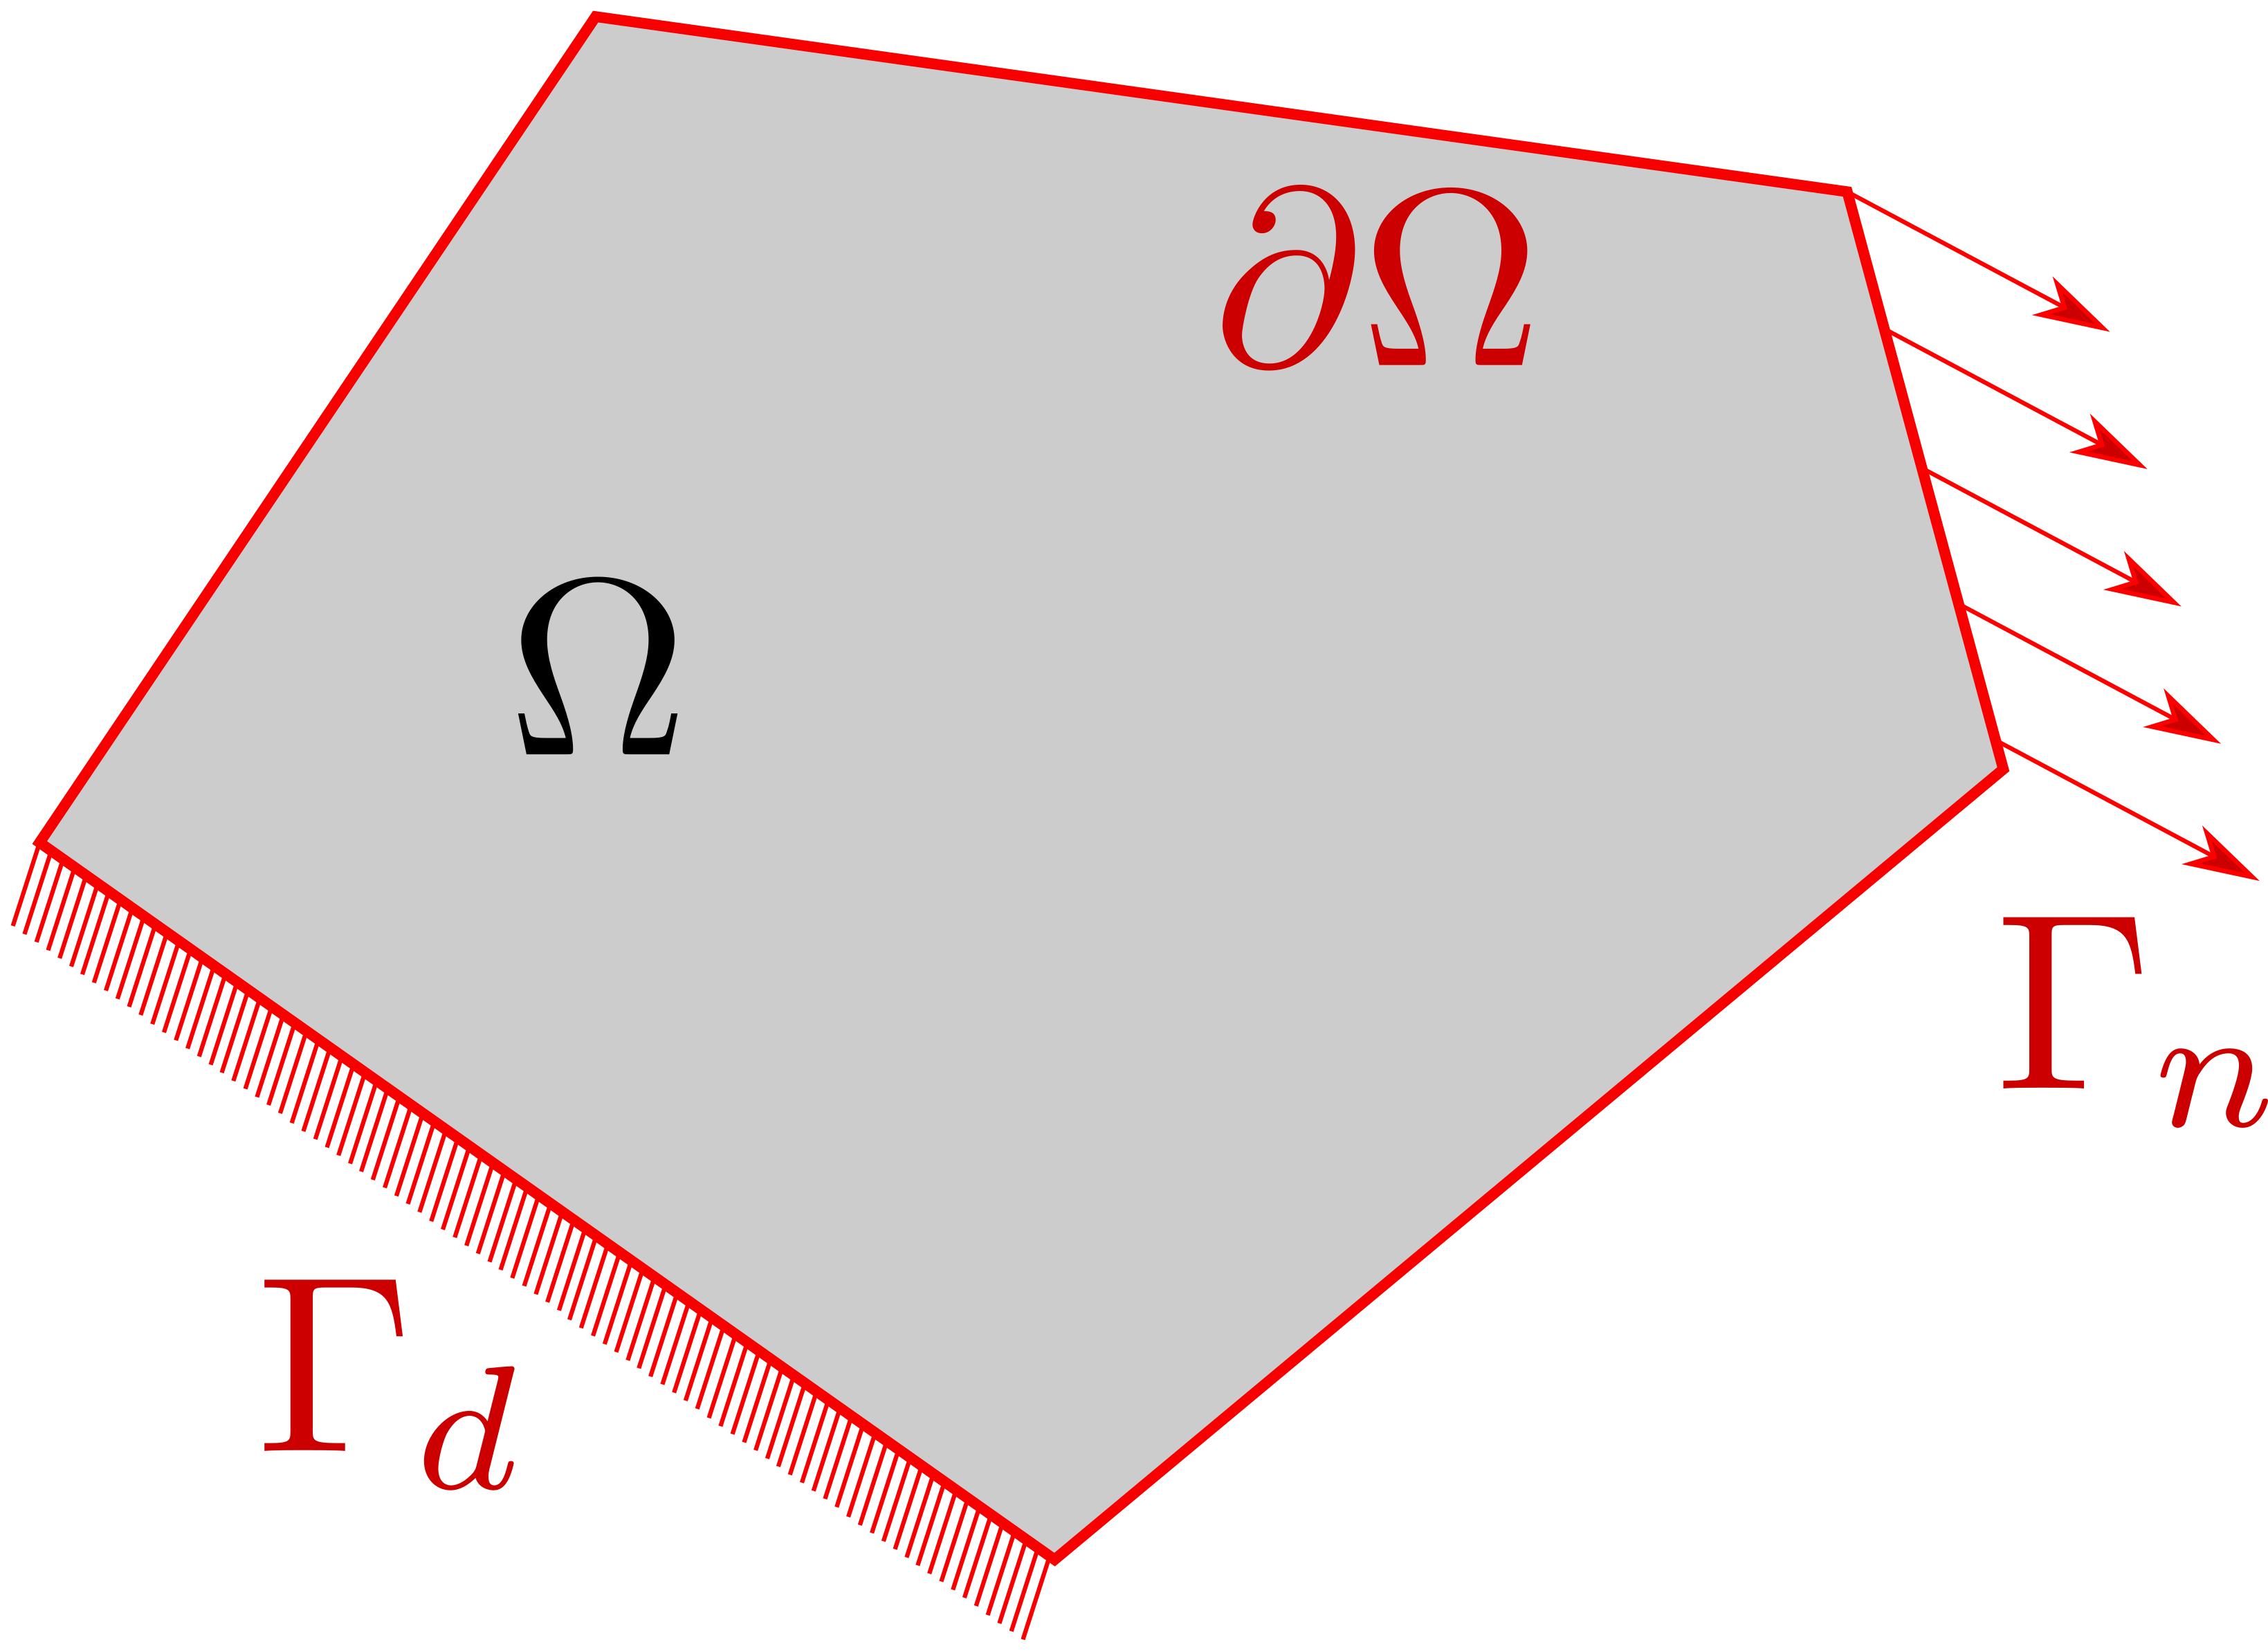
\includegraphics[width=\textwidth]{Figures/Continuum-solid}}
  \caption{Description of the boundary-value-problem in a
    continuum. Red lines represents the closure $\partial \Omega$
    of the domain $\Omega$ represented in gray.}
  \label{fig:Continuum-solid}
\end{figure}
%%%%%%%%%%%%%%%%%%%%%%%%%%%%%%%%%%%%%%%%%%%%%%%%%%%%%%%%%%%%%%%%%%%%%%%%%%
In this context the field \gls{u} allows to describe the \textit{global state}
of the system. Now the variable $\phi =
(\tens{\varepsilon},\tens{\sigma})$ is defined as the set of \textit{local
  states} at any point of the continuum which can be derived from the
field \gls{u} through the following set of governing equations and
restrictions that must be satisfied. First (i) we will relate
  global to local state by the \textit{compatibility equation}, where the the strain field \gls{strain} is extracted from \gls{u} is defined as:
\begin{equation}
  \label{eq:Compatibility-equation}
  \tens{\varepsilon} = \GradS{\vec{u}},
\end{equation}
together with essential or \acrfull{dbc} \gls{dirichlet-boundary}. We will further assume that 
strains are 
infinitesimal, therefore second order terms
in the spatial derivatives can be neglected. From here, the
stress field \gls{stress} will be considered the corresponding
conjugate variable for the strain field, being the one which
satisfies (ii) the \textit{conservation of lineal momentum equation}:
\begin{equation}
  \label{eq:Balance-momentum}
\rho \frac{D\vec{v}}{Dt} = \Div{\tens{\sigma}} + \rho \vec{b}
\end{equation}
together with the natural of \acrfull{nbc} \gls{neumann-boundary}.  An aditional component will be (iii) the constitutive equation as a linear
application from $\mathbb{R}^n$ to $\mathbb{R}^n$, which relate stress and strain increments as,
\begin{equation}
  \label{eq:Constitutive-equation}
\tens{\sigma} = \tens{D} \colon \tens{\varepsilon}.
\end{equation}
In this research, plane strain Linear Elasticity has been
  considered. Thus the constitutive tensor, \tens{D}, is the well
  known linear elastic one. The final equation of the set is (iv) the mass
conservation, which can be obtained by setting to zero the total derivative of the density field,
\begin{equation}
  \label{eq:Rho-material-derivative}
  \frac{D \rho}{D t} = \dot{\rho} + \rho \Div{\vec{v}} = 0.
\end{equation}

In order to obtain the variational statement of the problem, let us define a
virtual displacement field such that
\begin{equation}
  \label{eq:Hilbert-space}
  \vec{u}^{\psi} \in \mathcal{H}^1_0(\Omega) = \{ \vec{u}^{\psi} \in
  \mathcal{H}^1 \mid \vec{u}^{\psi} = \vec{0}\ \text{on}\ \Gamma_d \};
\end{equation}
in which the Cauchy sequences are convergent in \gls{domain} as well:
\begin{equation}
  \label{eq:cauchy-secuence}
  \Integral{3}{\vec{u}^{\psi}} < \infty\ \quad\text{and}\quad
  \Integral{3}{\tens{\varepsilon}^{\psi}} < \infty.
\end{equation}
The principle of virtual work states that the equilibrium solution to
the boundary-value problem of elasticity is the function $\vec{u} \in
\mathcal{H}^1_0$ such that, for any $\vec{u}^{\psi} \in
\mathcal{H}^1_0$,
the following holds:
%%%%%%%%%%%%%%%%%%%%%
\begin{equation}
  \label{eq:BalanceMomentum_wf}
  \Integral{3}{\rho\ \left( \frac{d\vec{v}}{dt}\ - \vec{b} \right) \cdot \vec{u}^{\psi}} =
  \Integral{2}{\vec{t}\ \cdot \vec{u}^{\psi}} - \Integral{3}{\tens{\sigma} \colon
   \tens{\varepsilon}^{\psi}}.
\end{equation}\\
%%%%%%%%%%%%%%%%%%%%%
Thus, equation~\eqref{eq:BalanceMomentum_wf}, together with
\eqref{eq:Constitutive-equation} and
\eqref{eq:Rho-material-derivative}, represents the weak form
formulation of the problem. Next, we will discretise the set of equations of the mathematical model using a double discretisation procedure, see figure~\ref{fig:MPM-discretization}.\\

\MODIFIED{First, the velocity field and the virtual displacements fields are discretised in a finite set of nodes $\textbf{X} = \{ \vec{x}_I, I \in \mathcal{B} \} \subset \mathbb{R}^n$, where $\mathcal{B} = 1, \ldots, N_I$. The continuum field can be reconstructed with the help of nodal values and an appropriate interpolation function $N_I(\vec{x})$. Also spatial derivatives of those quantities, such as gradients and divergences, are computed through the support of the background set of nodes as}
\begin{align}
    \label{eq:variable_reconstruction}
    \varphi(\vec{x}) &= \sum_{I\ \in\ \mathcal{B}} N_I(\vec{x})\ \varphi_I \\
    \label{eq:grad_variable_reconstruction}
    \Grad{\varphi}(\vec{x}) &= \sum_{I\ \in\ \mathcal{B}} \Grad{N_I(\vec{x})}\ \varphi_I
\end{align}
\MODIFIED{Secondly, the continuum \gls{domain} is discretised with a finite set of material points (also denominated particles the manuscript) $\hat{\Omega} = \{ \vec{x}_p, p \in \mathcal{C} \} \subset \Omega$, where $\mathcal{C} = 1, \ldots, N_p$. Any particle field such as position, velocity, mass, volume and stress denoted by $\vec{x}_p$, $\vec{v}_p$, $m_p$, $V_p$ and $\tens{\sigma}_p$ respectively are assigned to each material point. Furthermore, any particle field $\varphi_p$ can be reconstructed within the nodes in the neighbourhood of each particle, $\mathcal{B}_p \subset \mathcal{B}$, and evaluating the interpolation function in the position of each particle as}
\begin{align}
    \label{eq:particle_variable_reconstruction}
\varphi_p &= \sum_{I\ \in\ \mathcal{B}_p} N_I(\vec{x}_p)\ \varphi_I \\
\Grad{\varphi_p} &= \sum_{I\ \in\ \mathcal{B}_p} \Grad{N_I(\vec{x}_p)}\ \varphi_I
\end{align}
\MODIFIED{Regarding numerical integration, the material derivatives are evaluated using the Riemann integral definition \cite{Riemann_1854} applied to a finite set of points which associated volumes $V_p$ are interpreted as quadrature weights.}
\begin{equation}
    \label{eq:particle_riemann_integral}
\Integral{3}{\varphi} = \sum_{p\ \in\ \mathcal{C}} \varphi_p\ V_p 
\end{equation}

%%%%%%%%%%%%%%%%%%%%%%%%%%%%%%%%%%%%%%%%%%%%%%%%%%%%%%%%%%%%%%%%%%%%%%%%%%
\begin{figure}
%\sidecaption
  \centering
  \resizebox{0.5\hsize}{!}{
    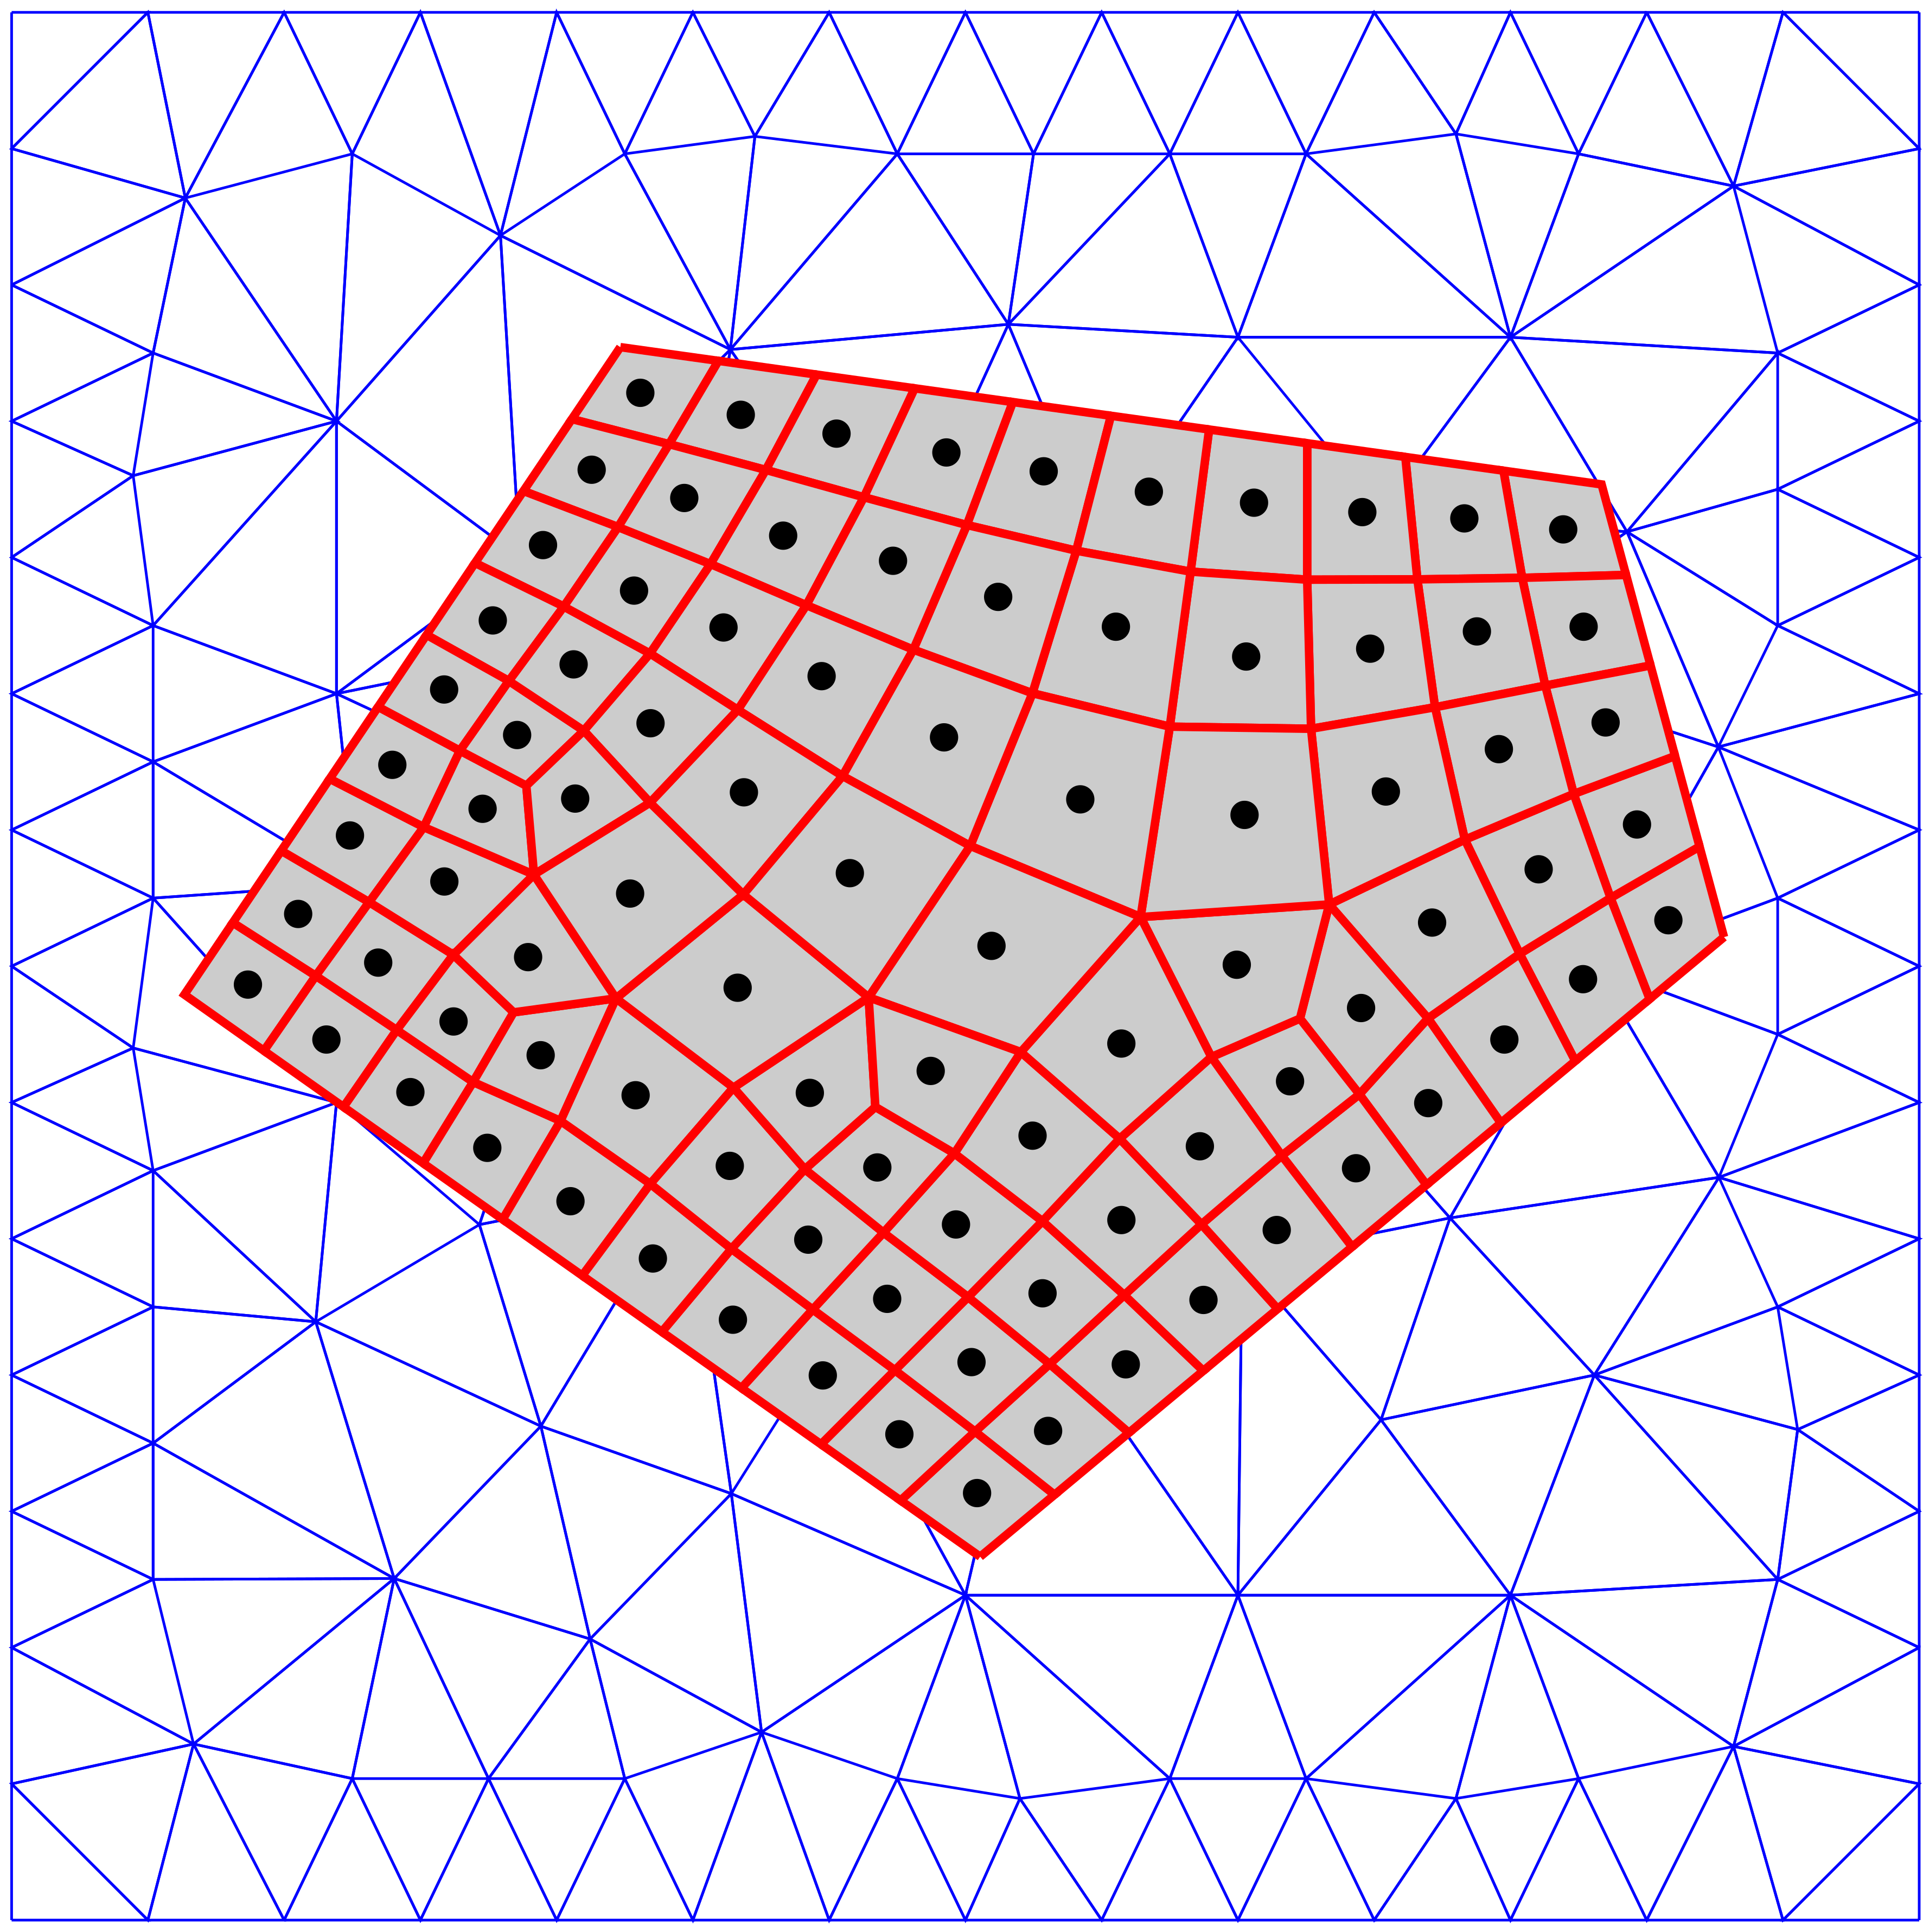
\includegraphics[width=\textwidth]{Figures/Mesh-particles-back}}
  \caption{Description of the spatial discretisation for domain presented in the
    figure~\ref{fig:Continuum-solid}. Blue mesh represent the
    background computational support, and the red mesh conforms the
    discretised continuum body.}
  \label{fig:MPM-discretization}
\end{figure}
%%%%%%%%%%%%%%%%%%%%%%%%%%%%%%%%%%%%%%%%%%%%%%%%%%%%%%%%%%%%%%%%%%%%%%%%%%
\MODIFIED{Let us illustrate the procedure described above by fully developing the term of the acceleration forces in \eqref{eq:BalanceMomentum_wf}. Employing the definition \eqref{eq:variable_reconstruction}, the velocity and virtual displacement fields can be approximated within its nodal values. Hence, the acceleration forces is reduced to}
\begin{equation}
    \label{eq:particle_acceleration_forces_I}
    \sum_{I,J\ \in\ \mathcal{B}} \Integral{3}{ \rho\ N_J(\vec{x})  \frac{d\vec{v}_J}{dt}\ \cdot N_I(\vec{x})\vec{u}_I^{\psi}}.
\end{equation}
\MODIFIED{Rearranging terms in \ref{eq:particle_acceleration_forces_I}, and subtracting from the integral those discrete variables, the following expression is obtained}
\begin{equation}
    \label{eq:particle_acceleration_forces_II}
    \sum_{I,J\ \in\ \mathcal{B}} \vec{u}_I^{\psi} \cdot \Integral{3}{ N_I(\vec{x})\ \rho\ N_J(\vec{x})}\ \frac{d\vec{v}_J}{dt}.
\end{equation}
\MODIFIED{Now, introducing the particle integral definition \eqref{eq:particle_riemann_integral} to compute the integral of \eqref{eq:particle_acceleration_forces_II}, and simplifying the it, is possible to achieve a discrete expression o the acceleration forces term as}
%%%%%%%%%%%%%%%%
\begin{equation}
\label{eq:particle_acceleration_forces_III}
\begin{split}
&\sum_{I,J\ \in\ \mathcal{B}} \vec{u}_I^{\psi} \cdot \sum_{p\ \in\ \mathcal{C}} N_{Ip}\ \rho_p\ N_{Jp}\ V_p\ \frac{d\vec{v}_J}{dt} = \\
&= \sum_{I,J\ \in\ \mathcal{B}} \vec{u}_I^{\psi} \cdot \sum_{p\ \in\ \mathcal{C}} N_{Ip}\ m_p\ N_{Jp}\ \frac{d\vec{v}_J}{dt} = \\
&= \tens{m}_{IJ}\ \frac{d\vec{v}_J}{dt}
\end{split}
\end{equation}
%%%%%%%%%%%%%%%%
\MODIFIED{$\tens{m}_{IJ}$, is the nodal mass matrix, and $N_{Ip}, N_{Jp}$ are the interpolation functions for nodes $I,J$ evaluated in the position of each particle $p$. In order to improve the computational efficiency and stability, the nodal mass matrix can be substituted by the lumped mass matrix $\tens{m}_{IJ}^{lumped}$. The remaining terms of \eqref{eq:BalanceMomentum_wf} are obtained within a similar procedure and can be found in literature, see for instance \cite{Zhang_book_2016}.
So equation \eqref{eq:BalanceMomentum_wf} has been discretised as}
%%%%%%%%%%%%%%%%%%%%%
\begin{equation}
\label{eq:BalanceMomentum_wf_discretized}
    \tens{m}_{IJ}\ \frac{d\vec{v}_J}{dt} = \sum_{p\ \in\ \mathcal{C}} - \tens{\sigma}_{p} \cdot \Grad{N_{Ip}} \frac{m_p}{\rho_p} + N_{Ip}\ \vec{b}_{p}\ m_p  + N_{Ip}\ \vec{t}^s_{p}\ m_p h^{-1}
\end{equation}
%%%%%%%%%%%%%%%%%%%%%
\MODIFIED{Where $h$ is the soil thickness in 2D, and $\tens{\sigma}_{p} = \tens{\sigma}_{p}(\tens{\varepsilon}_{p})$
is the particle $p$ stress field, which can be integrated employing
the suitable constitutive model. The particle strain field is approximated thorough the time integration of the rate of stress tensor, which is computed employing the velocity at the background set of nodes by the equation}
%%%%%%%%%%%%%%%%%%%%%
\begin{equation}
  \label{eq:IncrStrainPoint}
  \dot{\tens{\varepsilon}_{p}} = \frac{\Delta
    \tens{\varepsilon}_{p}}{\Delta t} = \sum_{I\ \in\ \mathcal{B}_p}
  \frac{1}{2} \left[\Grad{N_{Ip}}\ \otimes \vec{v}_{I} + \vec{v}_{I} \otimes
    \Grad{N_{Ip}}\ \right].
\end{equation}
%%%%%%%%%%%%%%%%%%%%%
Finally, mass conservation is guaranteed by enforcing the null value of
the material derivative of the density field $\frac{D \rho}{D t} = 0$.
This leads to a suitable equation to update the density field:
\begin{equation}
  \label{eq:MassConservation}
\dot{\rho} = - \rho\ \mathit{trace} \left( \dot{\tens{\varepsilon}} \right).
\end{equation}
Observe that to solve the equation \eqref{eq:BalanceMomentum_wf_discretized}, a second order time integration scheme is required. Therefore, time is
discretised into a finite set of time steps $k = 1\ldots ,Nt$, where $k$ is the current time step and $N_t$ is the total number of time steps. Once the nodal equilibrium equation is solved, the values at the nodes are interpolated back into the particles, which are advected
to the new position through:
\begin{equation}
  \label{eq:Updated_Lagrangian}
  \dot{\vec{v}}_p = \sum_{I\ \in\ \mathcal{B}_p} N_{Ip}\ \vec{a}_{I},\quad \text{and} \quad
  \dot{\vec{x}}_{p} = \sum_{I\ \in\ \mathcal{B}_p} N_{Ip}\ \vec{v}_{I}.  
\end{equation}
Traditionally, Eqs. \eqref{eq:BalanceMomentum_wf_discretized} and ~\eqref{eq:Updated_Lagrangian},
are solved with an explicit forward Euler algorithm. In the following subsection, this and the proposed schemes are described.

\subsection{MPM time integration scheme: the Newmark Predictor-Corrector proposal}
%\subsection{Explicit predictor-corrector scheme for \acrshort{mpm}.}
\label{sec:epc-algor-mpm}

As was stated previosuly, an explicit forward Euler algorithm has been utilized widely within the \acrshort{mpm} methodology. This scheme has been described in detail by many researchers
\cite{Sulsky1994}, \cite{Bardenhagen2002}, \cite{thesis_Andersen_2009} and can be sketched by the scheme of the figure~\ref{fig:MPM_algorithm}.
%%%%%%%%%%%%%%%%%%%%%%%%%%%%%%%%%%%%%%%%%%%%%%%%%%%%%%%%%%%%%%%%%%%%%%%%%%
\begin{figure}
%\sidecaption
  \centering
  \resizebox{0.8\hsize}{!}{
    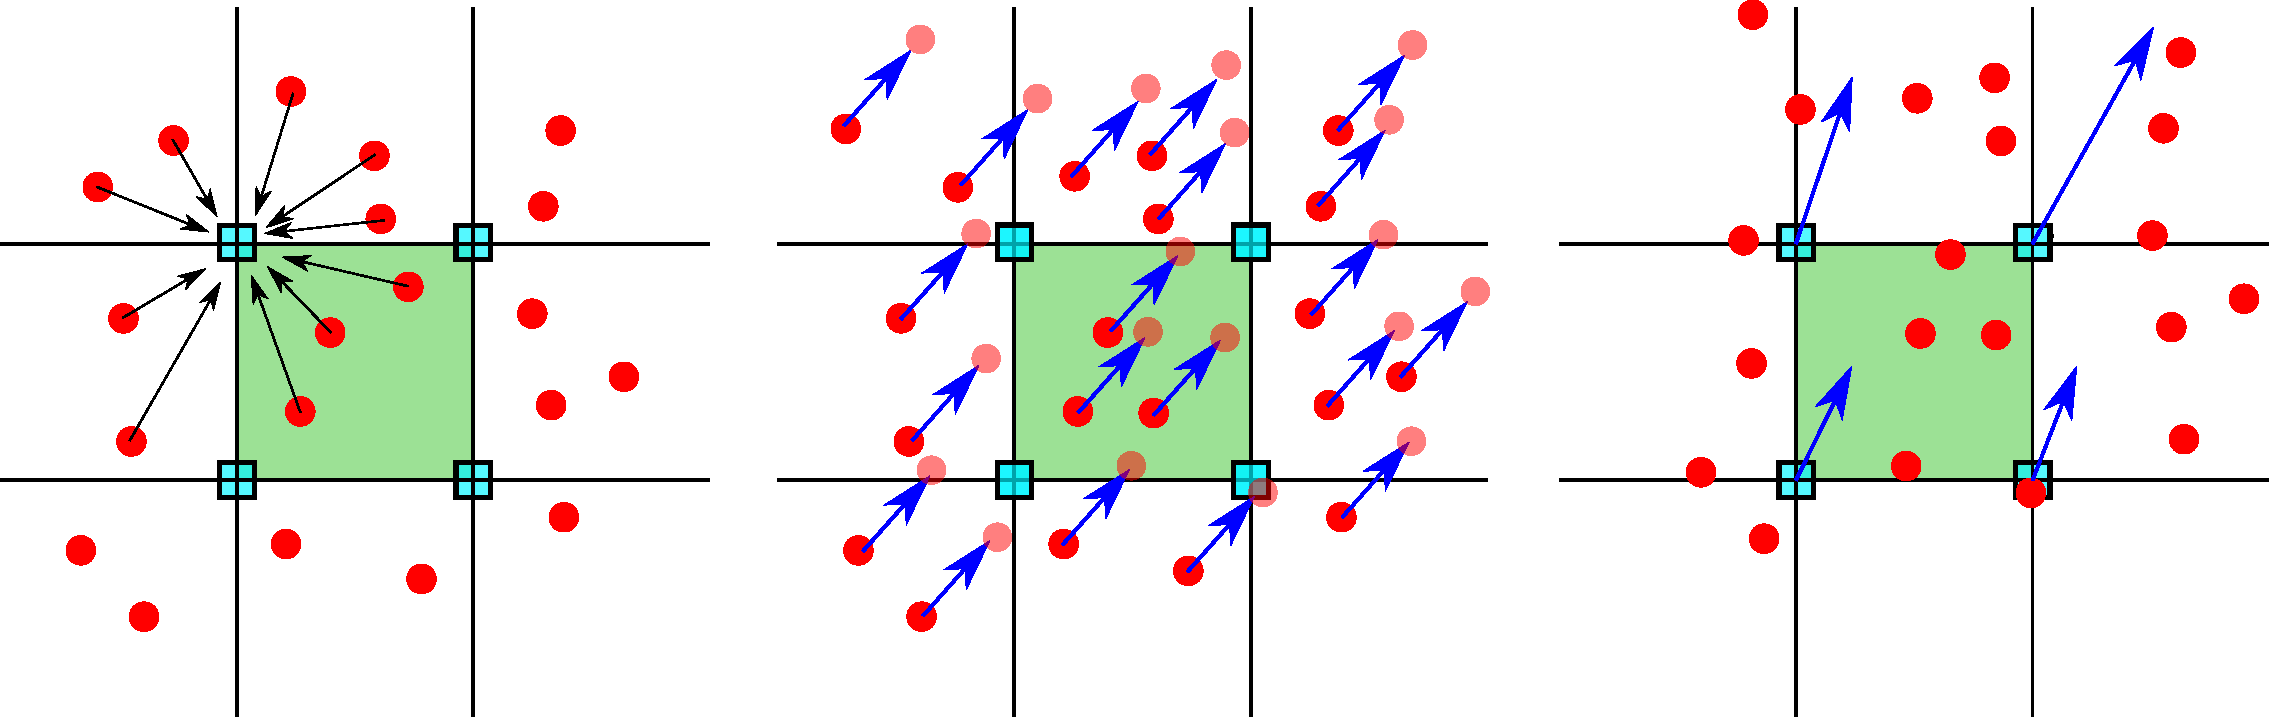
\includegraphics[width=\textwidth]{./Figures/MPM_scheme_horizontal}
  }
  \caption{Description of the three steps in \acrshort{mpm} standard algorithm.}
  \label{fig:MPM_algorithm}
\end{figure}
%%%%%%%%%%%%%%%%%%%%%%%%%%%%%%%%%%%%%%%%%%%%%%%%%%%%%%%%%%%%%%%%%%%%%%%%%%
Other authors have proposed many others time integration alternatives
like \cite{Guilkey_2003,Charlton_2017,Tran2019e}. In the
first publication on \acrshort{mpm} \cite{Sulsky1994}, the nodal acceleration
was employed to update the particles as
\begin{equation}
  \label{eq:Sulsky-1994-UL-v}
  \vec{v}_p^{k+1} = \vec{v}_p^{k} + \sum_{I\ \in\ \mathcal{B}_p} \Delta t\ N_{Ip}^{k}\ \vec{a}_{I}^{k},
\end{equation}
\begin{equation}
  \label{eq:Sulsky-1994-UL-x}
  \vec{x}_p^{k+1} = \vec{x}_p^{k} + \sum_{I\ \in\ \mathcal{B}_p} \Delta t\ N_{Ip}^{k}\ \vec{v}_{I}^{k}.
\end{equation}
However, as Andersen (2009)\cite{thesis_Andersen_2009} pointed out, this algorithm has been shown to be numerically unstable due to that
$\vec{f}_I^{int,k}$ can be infinite for an infinitesimal nodal mass
$\tens{m}_I$. This issue may lead to numerical problems when nodal acceleration
is obtained in the evaluation of the Eqs. \eqref{eq:Sulsky-1994-UL-x} and \eqref{eq:Sulsky-1994-UL-v}. Hence, a
corrected version of this algorithm was proposed by Zhang {\it et al.}
(2016)\cite{Zhang_book_2016}:
\begin{equation}
  \label{eq:Zhang-2016-UL-x}
  \vec{x}_p^{k+1} = \vec{x}_p^{k} + \sum_{I\ \in\ \mathcal{B}_p} \Delta t\ \frac{N_{Ip}^{k}\ \vec{p}_{I}^{k}}{\tens{m}_I}, 
\end{equation}
\begin{equation}
  \label{eq:Zhang-2016-UL-v}
  \vec{v}_p^{k+1} = \vec{v}_p^{k} + \sum_{I\ \in\ \mathcal{B}_p} \Delta t\ \frac{N_{Ip}^{k}\ \vec{f}_{I}^{k}}{\tens{m}_I}.
\end{equation}
Delving into the improvement of the accuracy of the \acrshort{mpm} explicit schemes, Tran \& Solowski (2019)\cite{Tran2019e} presented a
generalized-$\alpha$ scheme for \acrshort{mpm} inspired in the explicit time
integration algorithm proposed by Chung \& Hulbert
(1993)\cite{Geranlized_alpha_1993}, but with the particularity that
the acceleration is evaluated both in the beginning and the end of the
time step.
\begin{equation}
  \label{eq:Tran-2019-GA-v}
  \vec{v}_p^{k+1} = \vec{v}_p^{k} + \sum_{I\ \in\ \mathcal{B}_p} \Delta t\  N_{Ip}^{k}\ \left[(1 - \gamma)\ \vec{a}_I^{k} +
    \gamma\ \vec{a}_I^{k+1} \right],\\
\end{equation}
\begin{equation}
\label{eq:Tran-2019-GA-x}
  \vec{x}_p^{k+1} = \vec{x}_p^{k} + \sum_{I\ \in\ \mathcal{B}_p} N_{Ip}^{k} \left[ \Delta t\ \vec{v}_{I}^{k}+ \Delta t^2\left( (\frac{1}{2} - \beta)\
    \vec{a}_{I}^{k} + \beta\ \vec{a}_{I}^{k+1} \right) \right],
\end{equation}
\begin{equation}
  \label{eq:Tran-2019-GA-a}
  \vec{a}_p^{k+1} = \sum_{I\ \in\ \mathcal{B}_p} N_{Ip}^{k}\ \vec{a}_{I}^{k+1}.
\end{equation}

This scheme has been proven to damp out the highest frequency noises
\cite{Tran2019e}. However, it can present the same numerical instabilities
as in \eqref{eq:Sulsky-1994-UL-x},\eqref{eq:Sulsky-1994-UL-v} when
nodal masses become infinitesimal, and requires extra storage for
nodal values of acceleration and previous steps.

In this section, an explicit predictor-corrector time integration
scheme is proposed. It is based on the Newmark central differences
explicit scheme, which is also referred to as a-form 
$\gamma = 0.5$ and $\beta = 0$. This method is devoted to solve a system of equations of the type
\begin{equation*}
 \sum_{J\ \in\ \mathcal{B}} \Matrix{M}_{IJ}\ddot{\Vector{d}}_{J} + \Matrix{C}_{IJ}\dot{\Vector{d}}_{J} +
  \Matrix{K}_{IJ}\Vector{d}_{J} = \Vector{F}_{I}.
\end{equation*}
The nodal \acrshort{mpm} stage allows to apply this method
within the \acrshort{mpm} framework in a similar manner that the one
proposed by Tran~\textit{et al.}~\cite{Tran2019e}. By using the predictor definition, it is possible to calculate nodal velocities and update particles position employing nodal values
of velocity and acceleration. 

The predictor-corrector algorithm has
been described in the classic literature \cite{Hughes2000}, and its
stability and computational advantages were widely validated by Liu
\cite{Xiaojian94}. The ``classic'' \acrfull{npc} algorithm starts with a
predicted value of the nodal velocities at the $(k+1)$th time step, denoted by $\vec{\tilde{v}}_I^{k+1}$, which is calculated as follows:
\begin{equation}
  \label{eq:Predictor-velocity-I}
  \vec{\tilde{v}}_I^{k+1} = \vec{v}_I^k + (1 - \gamma)\ \Delta t\ \vec{a}_I^k.
\end{equation}

The \textit{user-defined}
parameter $\gamma \geq 0$ that appears in In \eqref{eq:Predictor-velocity-I}, influences both the predictor accuracy
and the stability of the algorithm. As pointed out Liu
\cite{Xiaojian94}, the truncation error of the predictor formula is
$O(\Delta t^3)$ when $\gamma = 0.5$, and is unconditionally stable if
$ 0 < \gamma \leq 0.25$.

To accommodate this step to \acrshort{mpm} framework, it is necessary to get
the nodal values of the velocity and acceleration throughout a variational
recovery process where particles quantities are transferred to the
mesh nodes. This technique arises as a generalization of the super-convergent recovery
procedures described by Zienkiewicz \& Zhu \cite{ZZ1992_I} (\textit{ZZ})
in the context of \acrshort{fem}. In \acrshort{mpm}, Gauss quadratures are not employed. However, 
integrals are computed following the Riemann integral definition,
where each component of the summation corresponds to a particle of the
discretisation. Also Bardenhagen \& Kober \cite{Bardenhagen2004}
proved that through this information-transference technique mass and momentum are conserved. So for a general particle variable $\Phi_p$, employing the
\textit{ZZ} technique, it is possible to get its nodal homologous $\Phi_I$  as:
\begin{equation}
  \label{eq:Variational-recovery}
   \Phi_I = \sum_{p\ \in\ \mathcal{C}} \frac{m_p N_{Ip} \Phi_p}{m_I}.
 \end{equation}
 Therefore, to get an analogous expression for
 \eqref{eq:Predictor-velocity-I} in the context of \acrshort{mpm}, the
 procedure described in the equation \eqref{eq:Variational-recovery}
 is employed, obtainen the following expression:
 \begin{equation}
   \label{eq:Predictor-velocity-II}
   \vec{\tilde{v}}_I^{k+1} = \sum_{p\ \in\ \mathcal{C}} \underbrace{\frac{N_{Ip}^{k} m_p
       \vec{v}_p^k}{m_I}}_{\vec{v}_I^{k}} + (1 - \gamma)\ \Delta t\  \underbrace{\frac{N_{Ip}^{k} m_p \vec{a}_p^k}{m_I}}_{\vec{a}_I^{k}}.
 \end{equation}
Nonetheless this way of computing the predictor stage can introduce
instabilities due to numerical cancellation likewise the original
Sulky algorithm. Thankfully, this can be avoided easily by the
equivalent formulation proposed as follows: 
\begin{equation}
  \label{eq:Predictor-velocity-II}
  \vec{\tilde{v}}_I^{k+1} =  \sum_{p\ \in\ \mathcal{C}} \frac{ N_{Ip}^{k} m_p (\vec{v}_p^k + (1 - \gamma)\ \Delta t\ \vec{a}_p^k)}{m_I}.
\end{equation}
This way of computing the nodal predictor is both numerically stable
and minimize the computational effort. Once nodal velocities are
obtained, the \acrshort{dbc} are imposed over \gls{dirichlet-boundary}. And in the
following, the ``classic'' \acrshort{mpm} algorithm continues to reach to the
equilibrium equation \eqref{eq:BalanceMomentum_wf_discretized}. Next, the
\textit{corrector} stage is introduced. As nodal
velocities were obtained earlier, this step is computed in the same way as
in \acrshort{fem},
\begin{equation}
  \label{eq:Corrector-velocity}
  \vec{v}_{I}^{k+1} = \vec{v}_{I}^{pred} + \gamma\ \Delta t\ \frac{\vec{f}_{I}^{k+1}}{\tens{m}_I^{k+1}}.
\end{equation}
Finally updated particle accelerations, velocities and positions are updated as,
\begin{align}
  \label{eq:Update-lagrangian-pce}
        &\vec{a}_p^{k+1} = \sum_{I\ \in\ \mathcal{B}_p} \frac{N_{Ip}^k\vec{f}_{I}^{k}}{\tens{m}_I^k}\\
      &\vec{v}_p^{k+1} = \vec{v}_p^n + \sum_{I\ \in\ \mathcal{B}_p} \Delta t\
        \frac{N_{Ip}^k\
        \vec{f}_{I}^{k}}{\tens{m}_I^k}\\
      &\vec{x}_p^{k+1} = \vec{x}_p^n + \sum_{I\ \in\ \mathcal{B}_p} \Delta t\
         N_{Ip}^k\ \vec{v}_{I}^{k} +
        \frac{1}{2}\Delta t^2\ \frac{N_{Ip}^k\
        \vec{f}_{I}^{k}}{\tens{m}_I^k}.
\end{align}
Notice that particle displacements are computed using the corrected
nodal velocities as well as the accelerations with the velocities
of the predictor. However, particle velocities and accelerations
are computed using the corrected velocities. Therefore here we share similarities
with the \textit{leapfrog scheme} where position is not updated at
full time step, but the velocity is updated at half time steps. Notice
also that, with this approach, the calculation of nodal momentum values
are not required. Due to its simplicity, the proposed scheme can be implemented with minor modifications over the standard forward Euler. The full implementation is summarized in the algorithm~\ref{algo:1}.

\begin{algorithm}
  \floatname{algorithm}{Algorithm 1}
  \renewcommand{\thealgorithm}{}
  \caption{\acrfull{npc} scheme} \label{algo:1}
  \begin{algorithmic}[1]
    %%%%%%%%%%%%%%%%%%%%%%%%%%%%%%%%%%%%%%%%%%%%%%%%%%%%%%%%%%%%%%%%%%%%%%%%%%%%%%%%%%%%%% º
    \STATE \textbf{Update mass matrix}.
    %%%%%%%%%%%%%%%%%%%%%%%%%%%%%%%%%%%%%%%%%%%%%%%%%%%%%%%%%%%%%%%%%%%%%%%%%%%%%%%%%%%%%% 
    \STATE \textbf{Explicit Newmark Predictor}:\\
    \begin{equation*}
      \vec{v}_I^{pred} = \sum_{p\ \in\ \mathcal{C}} \frac{ N_{Ip}^{k} m_p (\vec{v}_p^k + (1 - \gamma)\ \Delta t\ \vec{a}_p^k)}{m_I}.
    \end{equation*}
    %%%%%%%%%%%%%%%%%%%%%%%%%%%%%%%%%%%%%%%%%%%%%%%%%%%%%%%%%%%%%%%%%%%%%%%%%%%%%%%%%%%%%% 
    \STATE \textbf{Impose essential boundary conditions}:\\
    At the fixed boundary, set $\vec{v}_{I}^{pred} = 0$. 
    %%%%%%%%%%%%%%%%%%%%%%%%%%%%%%%%%%%%%%%%%%%%%%%%%%%%%%%%%%%%%%%%%%%%%%%%%%%%%%%%%%%%%% 
    % \STATE \textbf{Discard the previous nodal values}.
    %%%%%%%%%%%%%%%%%%%%%%%%%%%%%%%%%%%%%%%%%%%%%%%%%%%%%%%%%%%%%%%%%%%%%%%%%%%%%%%%%%%%%% 
    \STATE \textbf{Deformation tensor increment calculation}.
    \begin{equation*}
      \dot{\tens{\varepsilon}_{p}}^{k+1} = \sum_{I\ \in\ \mathcal{B}_p} \left[ \vec{v}_{I}^{pred} \otimes \Grad{N_{Ip}^{k+1}} \right]^s\ \quad \text{and}\ \quad \Delta \tens{\varepsilon}_{p}^{k+1} = \Delta t\ \dot{\tens{\varepsilon}_{p}}^{k+1}.
    \end{equation*}
    %%%%%%%%%%%%%%%%%%%%%%%%%%%%%%%%%%%%%%%%%%%%%%%%%%%%%%%%%%%%%%%%%%%%%%%%%%%%%%%%%%%%%% 
    \STATE \textbf{Update the density field}:
    \begin{equation*}
      \rho_p^{k+1} = \frac{\rho_p^k}{1 + \mathit{trace}\left[\Delta\tens{\varepsilon}_{p}^{k+1}\right]}.
    \end{equation*}
    %%%%%%%%%%%%%%%%%%%%%%%%%%%%%%%%%%%%%%%%%%%%%%%%%%%%%%%%%%%%%%%%%%%%%%%%%%%%%%%%%%%%%% 
    \STATE \textbf{Balance of forces calculation}:\\
    Calculate the total grid nodal forces by evaluating the right hand side of 
    \eqref{eq:BalanceMomentum_wf_discretized} in the time step $k+1$.
    In those nodes where $\Deriv{\vec{v}_I^{k}}{t} \big\rvert_{\Gamma_d} = 0$, the acceleration is fixed to zero and nodal forces are stored as reactions.\\
    %%%%%%%%%%%%%%%%%%%%%%%%%%%%%%%%%%%%%%%%%%%%%%%%%%%%%%%%%%%%%%%%%%%%%%%%%%%%%%%%%%%%%% 
    \STATE \textbf{Explicit Newmark Corrector}:
    \begin{equation*}
      \vec{v}_{I}^{k+1} = \vec{v}_{I}^{pred} + \gamma\ \Delta t\ \frac{\vec{f}_{I}^{k+1}}{\tens{m}_I^{k+1}}.
    \end{equation*}
    %%%%%%%%%%%%%%%%%%%%%%%%%%%%%%%%%%%%%%%%%%%%%%%%%%%%%%%%%%%%%%%%%%%%%%%%%%%%%%%%%%%%%%
    \STATE \textbf{Update particles lagrangian quantities}:
    \begin{align*}
      &\vec{a}_p^{k+1} = \sum_{I\ \in\ \mathcal{B}_p} \frac{N_{Ip}^k\vec{f}_{I}^{k}}{\tens{m}_I^k},\\
      &\vec{v}_p^{k+1} = \vec{v}_p^n + \sum_{I\ \in\ \mathcal{B}_p} \Delta t\
        \frac{N_{Ip}^k\
        \vec{f}_{I}^{k}}{\tens{m}_I^k},\\
      &\vec{x}_p^{k+1} = \vec{x}_p^n + \sum_{I\ \in\ \mathcal{B}_p} \Delta t\
         N_{Ip}^k\ \vec{v}_{I}^{k} +
        \frac{1}{2}\Delta t^2\ \frac{N_{Ip}^k\
        \vec{f}_{I}^{k}}{\tens{m}_I^k}.
    \end{align*}
    %%%%%%%%%%%%%%%%%%%%%%%%%%%%%%%%%%%%%%%%%%%%%%%%%%%%%%%%%%%%%%%%%%%%%%%%%%%%%%%%%%%%%% 
    \STATE \textbf{Reset nodal values}.
  \end{algorithmic}
\end{algorithm}

\subsection{Local \textit{Max-Ent} approximants}
\label{sec:local-max-ent}
The popularity of the \acrshort{mpm} has increased notoriously during
the recent years due to its ability to deal with large strain problems
without mesh distorsion issues inherent to mesh based methods like
\acrshort{fem}, see Wi{\c{e}}ckowski \cite{Wieckowski2004}. However, in the simulations
made with the original \acrshort{mpm}, numerical noises appear when particles
cross the cell boundaries. Solving this issue is the main goal of the employment of the \acrshort{lme} shape functions.

\acrfull{lme} approximation schemes were
first introduced by Arroyo \& Ortiz (2006)\cite{Arroyo2006} and has been
recently tested under \acrshort{mpm} framework by Wobbes {\it et al.}
(2020)\cite{Wobbes2020}. The simulations presented in \cite{Wobbes2020} of \acrshort{mpm}
within \acrshort{lme} show considerably more accurate stress
approximations than traditional \acrshort{mpm} schemes. However, 
how the regularization parameter $\beta$ affects to the accuracy and
stability of the solution is not assessed deeply in that research. The tuning of this $\beta$ parameter allows to make the comparison of the accuracy against analogous traditional \acrshort{mpm} shape function.

The basic idea of the shape functions based on such an estimate is to interpret the shape function $N_I(\vec{x})$ as a probability. This allows us to introduce two important limits:
the principle of maximum-entropy (\textit{max-ent}) statistical
inference stated by \cite{Jaynes1957}, and the Delaunay triangulation
which ensures the minimal width of the shape function. 

This approximation scheme represents an optimal compromise, in the sense of
Pareto, between the \textit{unbiased statistical inference} based on
the nodal data which leads to the principle of \textit{Maximum-Entropy}
stated by Jaynes \cite{Jaynes1957}, and the definition of local shape
functions of \textit{least width} the least biased shape functions.

Taking the definition of entropy as a measure of how uncertainty a
random variable is averaged on all its possible outcomes. And adopting
the Shannon's entropy as the starting point:
\begin{equation}
  \label{eq:Shannon-entropy}
  H(p_1(\vec{x}),\ldots,p_n(\vec{x})) = -\sum^{N_n}_{I=1}{p_I(\vec{x})\log p_I }
\end{equation}
where $p_I(\vec{x})$ is the probability, equivalent to the mentioned
shape function $N_I(\vec{x})$, satisfying both the zeroth and
first-order consistency. The least-biased approximation scheme is
given by
\begin{align*}
  \label{eq:least-biased-approximation-scheme}
  \text{(LME)} \hspace{0.15cm} &\text{Maximize} \hspace{0.15cm} H(N_I) \equiv
  -\sum_{I}^{N_n}{N_I(\vec{x})\log N_I }\\
  &\text{subject to}\
  \begin{cases}
    N_I \ge 0, \hspace{0.15cm} \text{I=1, ..., n} \\[1em]   
    \sum\limits_{I=1}^{N_n}{N_I} = 1 \\[1em]   
    \sum\limits_{I=1}^{N_n}{N_I \vec{x}_I} = \vec{x} \\
  \end{cases}
\end{align*}
On the other hand, the control of the shape function width and its
decay with distance away from the corresponding nodes is a desirable property. To reach to this objective \cite{Arroyo2006} propose the following linear program,
\begin{align*}
  %\label{eq:RAJAN}
  \text{(RAJ)} \hspace{0.15cm} &\text{For fixed} \hspace{0.15cm}
  \vec{x} \hspace{0.15cm} \text{minimize} \hspace{0.15cm} U(\vec{x}_p,N_I) \equiv
\sum_I N_I |\vec{x}_p - \vec{x}_I |^2\\
  &\text{subject to}\
  \begin{cases}
    N_I \ge 0, \hspace{0.15cm} \text{I=1, ..., n} \\[1em]   
    \sum\limits_{I=1}^{N_n}{N_I} = 1 \\[1em]   
    \sum\limits_{I=1}^{N_n}{N_I \vec{x}_I} = \vec{x} \\
  \end{cases}
\end{align*}
To reach to a compromise between two competing objectives, a Pareto set is defined by \cite{Arroyo2006} as,
\begin{align*}
  %\label{eq:LME-scheme-pareto-set}
  \text{(LME)}_{\beta} \hspace{0.15cm} &\text{For fixed} \hspace{0.15cm}
  \vec{x} \hspace{0.15cm} \text{minimize} \hspace{0.15cm} f_{\beta}(\vec{x}, N_I) \equiv \beta U(\vec{x},N_I) - H(N_I) \\
  &\text{subject to}\
  \begin{cases}
    N_I \ge 0, \hspace{0.15cm} \text{I=1, ..., n} \\[1em]   
    \sum\limits_{I=1}^{N_n}{N_I} = 1 \\[1em]   
    \sum\limits_{I=1}^{N_n}{N_I \vec{x}_I} = \vec{x} \\
  \end{cases}
\end{align*}
The regularization or \textit{thermalization} parameter
between the two criterion, $\beta$, has Pareto optimal values in the range
$\beta \in (0,\infty)$. The unique solution of
the local \textit{max-ent} problem \acrshort{lme}$_\beta$ is:
\begin{equation}
  \label{eq:LME-p}
N_I^*(\vec{x})=\frac{\exp\left[ -\beta \; |\vec{x}-\vec{x}_I|^2 +
    \vec{\lambda}^* \cdot (\vec{x}-\vec{x}_I) \right] } {Z(\vec{x},\vec{\lambda}^*)}
\end{equation}
where
\begin{equation}
  \label{eq:LME-Z}
Z(\vec{x}, {\vec{\lambda}}) = \sum_{I=1}^{N_n}{ \exp \left[ -\beta \; |\vec{x}-\vec{x}_I|^2 + \vec{\lambda} \cdot (\vec{x}-\vec{x}_I)  \right]}
\end{equation}
being $\vec{\lambda}^*(\vec{x})$ the unique minimiser for the function $\log
Z(\vec{x}, \vec{\lambda})$. The traditional way to obtain such a minimiser is using Eq.~(\ref{eq:LME-J}) to calculate small increments of $\partial\vec{\lambda}$ in a Newton-Raphson approach. $\tens{J}$ is defined as the Hessian matrix, obtained by:
\begin{eqnarray}
  \label{eq:LME-J} 
  \tens{J}(\vec{x}, \vec{\lambda},\beta) &\equiv& \frac{\partial
                                                  \vec{r}}{\partial \vec{\lambda}}\\
  \label{eq:LME-r}
  \vec{r}(\vec{x},\vec{\lambda},\beta) &\equiv& \frac{\partial \log{ Z(   \vec{x},\vec{\lambda}})}{\partial \vec{\lambda}}  = \sum_I^{N_n} p_I(\vec{x},\vec{\lambda},\beta) \, (\vec{x} - \vec{x}_I)
\end{eqnarray}
In order to obtain the first derivatives of the shape function, it is also necessary to compute~$\nabla N_I^*$
\begin{equation}
  \label{eq:LME-grad-p}
\nabla N_I^* = N^*_I  \, \left(\nabla f^*_I-\sum_J^{N_n} N^*_J \, \nabla f^*_J\right)
\end{equation}
where
\begin{equation}
  \label{eq:LME-f}
f^*_I(\vec{x},  \vec{\lambda},\beta)=-\beta \, |\vec{x}-\vec{x}_I|^2 + \vec{\lambda}   \,  (\vec{x}-\vec{x}_I)
\end{equation}
Employing the chain rule, rearranging and considering $\beta$ as a constant, Arroyo and Ortiz~\cite{Arroyo2006} obtained the following expression for the gradient of the shape function.
\begin{eqnarray}
\nabla N_I^* &=& -N_I^* \,  (\tens{J}^*)^{-1} \,  (\vec{x} - \vec{x}_I) \label{eq26} 
\end{eqnarray}
The regularization parameter $\beta$ of \acrshort{lme} shape functions may be
controlled by adjusting a dimensionless parameter, $\gamma=\beta h^2$
\cite{Arroyo2006}, where $h$ is defined as a measure of the nodal
spacing. 
Since $N_I$ is defined in the entire domain, in practice, the
function $\exp(-\beta \vec{r} )$ truncated  by  a given tolerance,
10$^{-6}$ in this research,  would ensure a reasonable range of
neighbours (see \cite{Arroyo2006} for details).
This tolerance defines the limit values of the influence radius and is used thereafter to
find the neighbour nodes of a given integration point. An additional remark is that, analogous to alternative non-polynomial meshfree basis functions, the \acrshort{lme} approximation scheme requires more than $d+1$ nodes to determine the values of the shape functions as well as their derivatives at any point in the convex hull of the nodal set, where $d$ is the dimension of the problem.

This interpolation technique avoids important shortcomings when using
\acrshort{gimp} or B-Spline \acrshort{mpm} regarding the computational domain boundaries
(see Steffen {\it et al.} (2008)\cite{Steffen2008b}), which are related to the
additional considerations in the application of the boundary
conditions. Motivated by their increased extents, particles may share an influence radius that lies outside of the simulation domain. Some researchers have solved this problem with the so called ``extra'' or ``ghost'' nodes. These nodes require especial treatment, similar
to those employed in the \acrfull{sph}, for
further details see Liu \& Liu (2003)\cite{Liu2003}. The approach here
described does not requires the employment of this artifices.
Due to the \acrshort{fem}-compatibility, the \acrshort{lme} shape
function is degenerated to linear finite element shape function if
$d+1$ neighbouring nodes are chosen as the support, where $d$ is the
number of dimensions in the problem. Ullah {\it et al.} \cite{Augarde_2013} took advantage of the \acrshort{lme} \acrshort{fem}-compatibility to couple the \acrfull{efgm} and \acrshort{fem} for linear elasticity and for problems with both material and geometrical non-linearities. Furthermore, with a conveniently
adopted \textit{regularization} parameter it is possible to get a 
\acrshort{gimp}-like shape function. Finally \acrshort{sph}-like
behaviour can be obtained for lower values of $\gamma$ since the
support of the shape function is drastically increased, and therefore
\textit{smoother} solutions are obtained. See \cite{Navas2016} for an
application of this capability, where oscillations due to
excess of pore water pressure in consolidation problems are smoothed
out by using this technique. The employment of smoothing algorithms is
also straightforward in the fluid-solid interaction problems
\cite{Arduino_2018}. A proof of this statements is observed in
figure~\ref{fig:LME_MPM}, where the \acrshort{lme} adaptability is illustrated.\\
%%%%%%%%%%%%%%%%%%%%%%%%%%%%%%%%%%%%%%%%%%%%%%%%%%%%%%%%%%%%%%%%%%%%%%%%%%
\begin{figure*}
  \centering
  \subfigure[Q4]{    
    \begin{tabular}{c}
      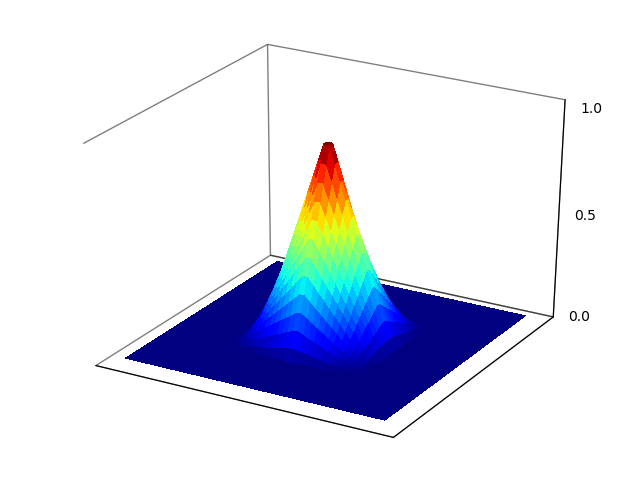
\includegraphics[width=0.14\textwidth]{Figures/MPM_Shape_Fun}\\
      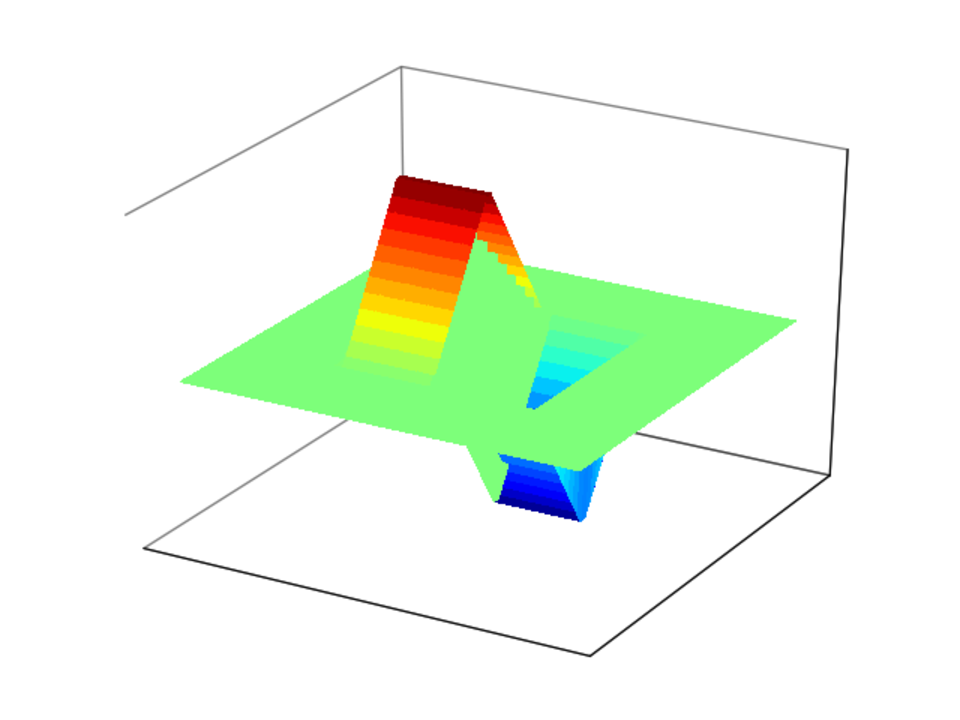
\includegraphics[width=0.14\textwidth]{Figures/MPM_Shape_Fun_dx}\\
      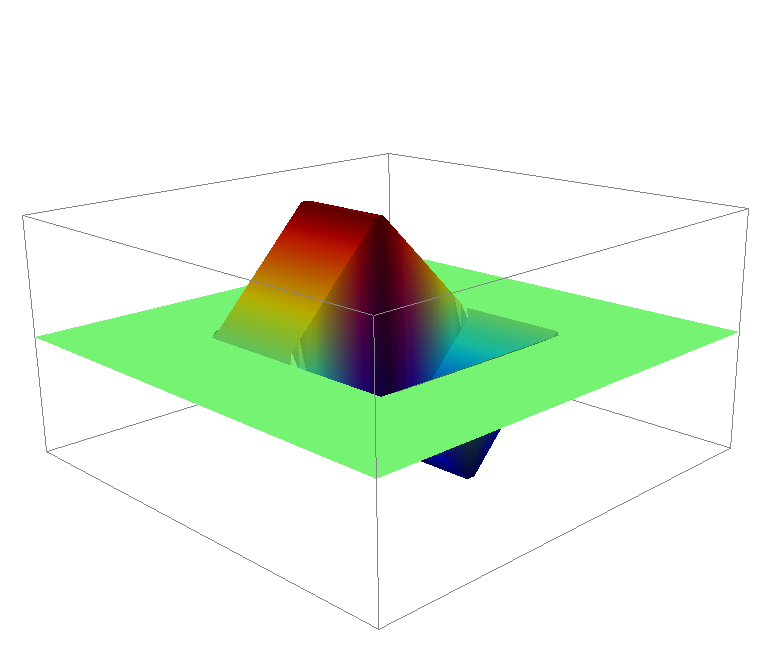
\includegraphics[width=0.14\textwidth]{Figures/MPM_Shape_Fun_dy}
    \end{tabular}
  }
  \subfigure[$\text{LME}_{17}$]{
    \begin{tabular}{c}      
      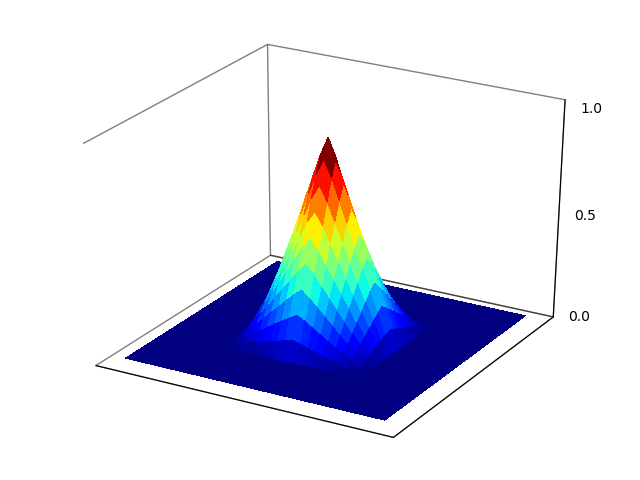
\includegraphics[width=0.14\textwidth]{Figures/LME_17_3_Shape_Fun}\\
      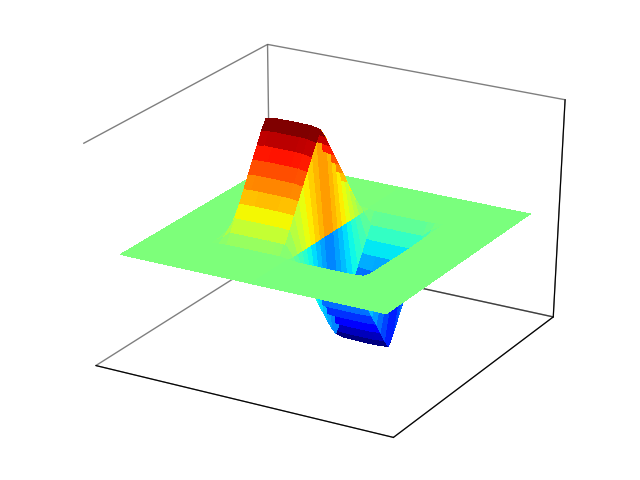
\includegraphics[width=0.14\textwidth]{Figures/LME_17_3_Shape_Fun_dx}\\
      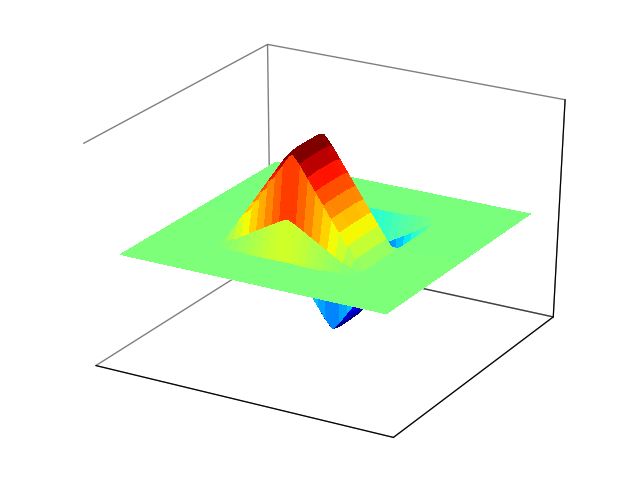
\includegraphics[width=0.14\textwidth]{Figures/LME_17_3_Shape_Fun_dy}
    \end{tabular}
  }
  \subfigure[uGIMP]{
    \begin{tabular}{c}
      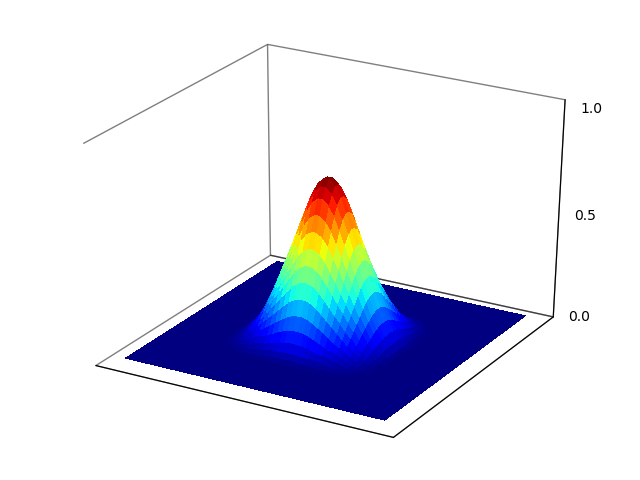
\includegraphics[width=0.14\textwidth]{Figures/GIMP_Shape_Fun}\\
      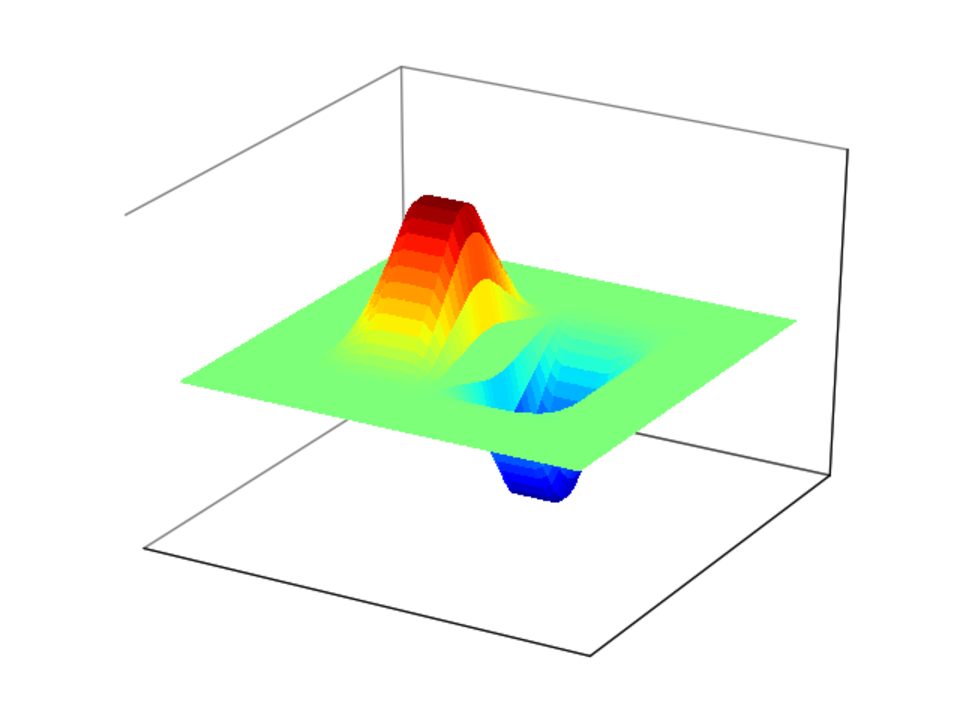
\includegraphics[width=0.14\textwidth]{Figures/GIMP_Shape_Fun_dx}\\
      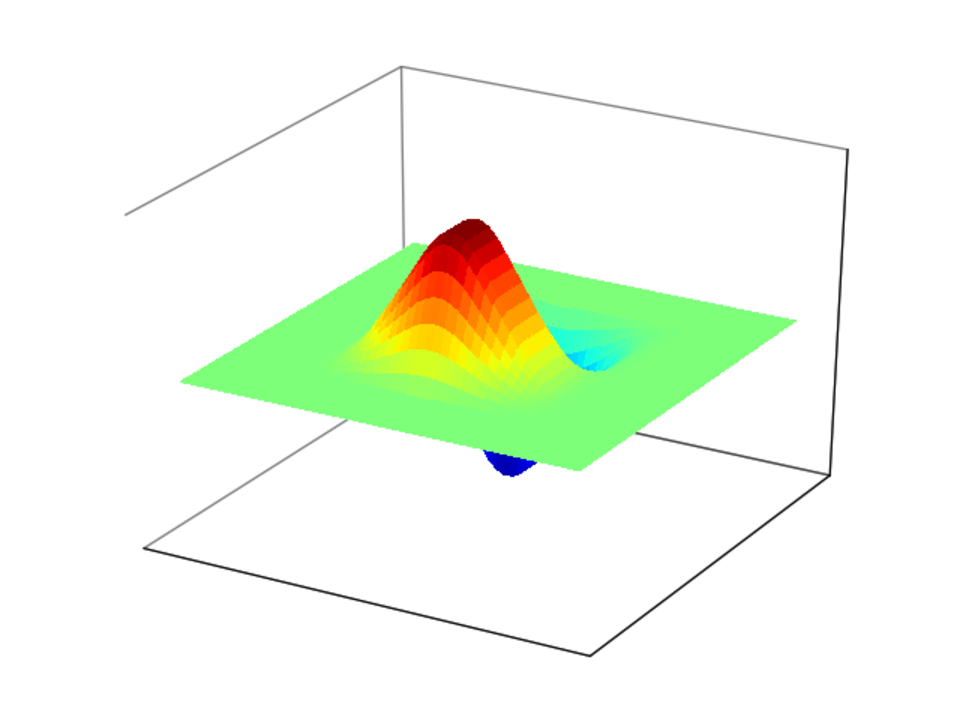
\includegraphics[width=0.14\textwidth]{Figures/GIMP_Shape_Fun_dy}
    \end{tabular}
  }
  \subfigure[$\text{LME}_{10}$]{
    \begin{tabular}{c} 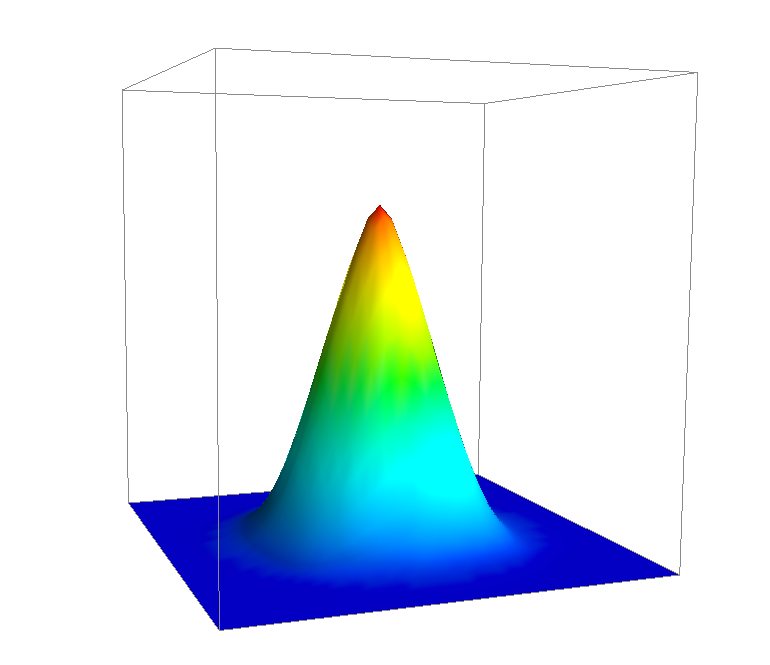
\includegraphics[width=0.14\textwidth]{Figures/LME_10_0_Shape_Fun}\\ 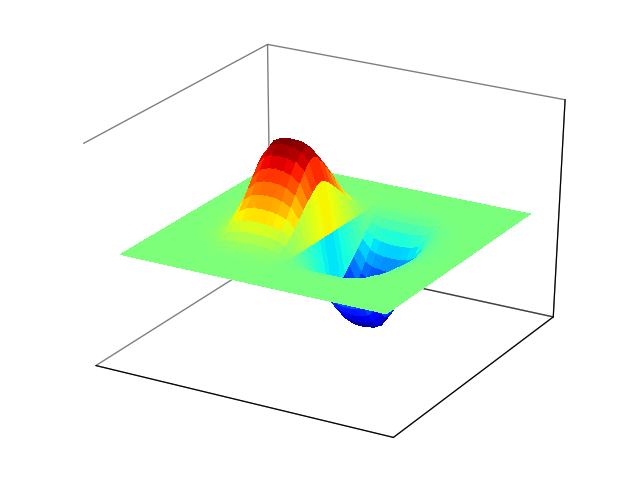
\includegraphics[width=0.14\textwidth]{Figures/LME_10_0_Shape_Fun_dx}\\      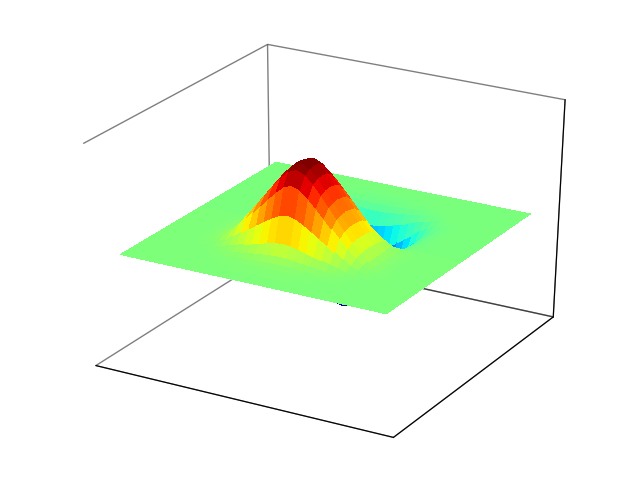
\includegraphics[width=0.14\textwidth]{Figures/LME_10_0_Shape_Fun_dy}    
    \end{tabular}
  }
  \subfigure[$\text{LME}_{5}$]{
    \begin{tabular}{c}
      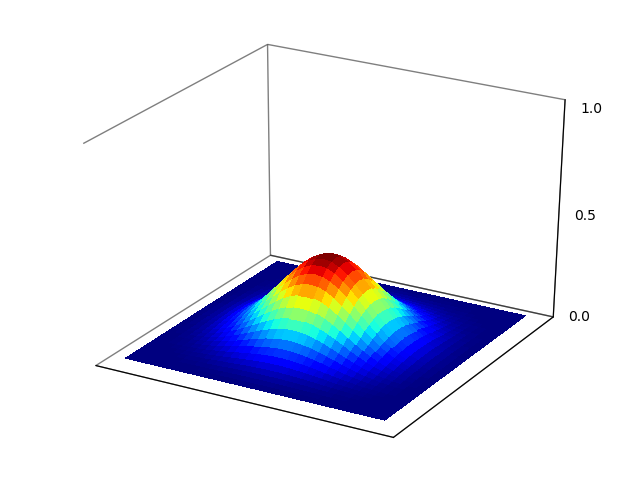
\includegraphics[width=0.14\textwidth]{Figures/LME_5_0_Shape_Fun}\\
      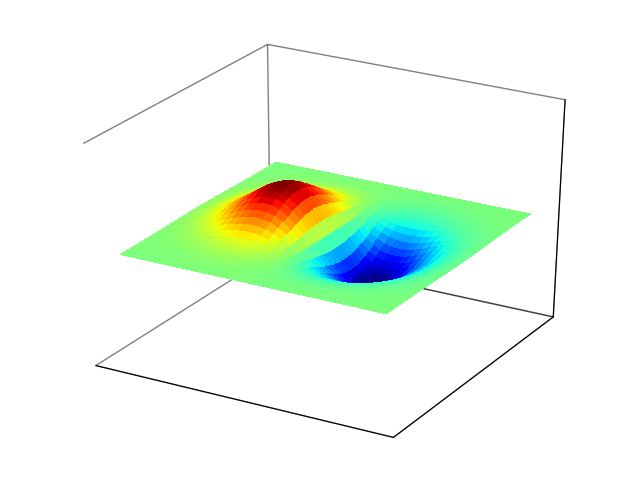
\includegraphics[width=0.14\textwidth]{Figures/LME_5_0_Shape_Fun_dx}\\
      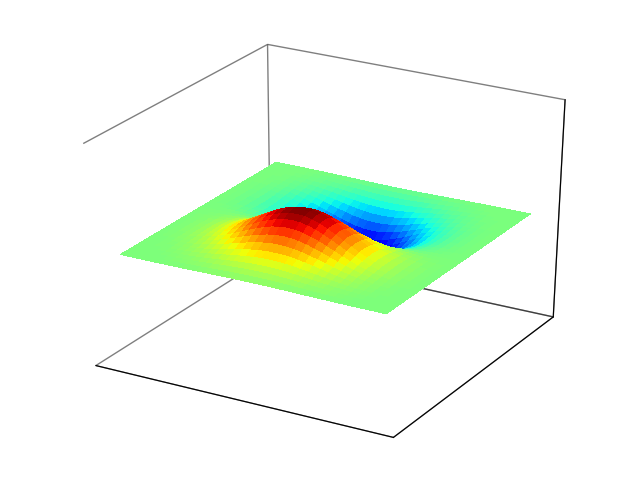
\includegraphics[width=0.14\textwidth]{Figures/LME_5_0_Shape_Fun_dy}
    \end{tabular}
  }
  \caption{Comparative of linear piecewise shape functions (Q4) and
    \acrshort{ugimp} shape functions \textit{versus}  \acrshort{lme}
    approximation for a two-dimensional arrangement of nodes, and
    spatial derivatives for several values of $\gamma = \beta/h^2$.}
  \label{fig:LME_MPM}
\end{figure*}
%%%%%%%%%%%%%%%%%%%%%%%%%%%%%%%%%%%%%%%%%%%%%%%%%%%%%%%%%%%%%%%%%%%%%%%%%% 
In this research and in \cite{Arroyo2006}, $\beta$ is a scalar as the
influence area of the shape function is controlled by the Euclidean
norm, therefore the search area is geometrically a circle in 2D, or a
sphere in 3D. Building upon the idea of anisotropic shape functions,
\cite{Kochmann2019} introduced an enhanced version of the original
\acrshort{lme} scheme, which uses an anisotropic support to deal with 
tensile instability. This is another benefit of the proposed methodology, that, although is out of the scope of the present document, will be incorporated in future research.

\MODIFIED{Unfortunately, the employment of \textit{max-ent} approximants is not free of pitfalls. Some requirements such as the need for a convex domain, as well as those derived from its calculation (the determination of the Lagrange Multipliers, specially at the boundaries, or the obtainment of the minimizer of the logarithmic function), make the usage of it a challenging tool. Concerning the convex domain requirement, Arroyo \& Ortiz~\cite{Arroyo2006} briefly discussed the existence of non-convex domains, and proposed some solutions to it. For instance, the possibility of replacing the Euclidean distance $\lVert x - x_a \rVert$ in the definition of the shape functions by the length of the shortest path contained within the domain connecting $x$ and $x_a$. Or by decomposing the non-convex domain into convex sub-domains.}

\MODIFIED{Of course the requirement of convex domain is not exclusive from \textit{max-ent}, it also concerns to the remaining interpolation techniques in the \acrshort{mpm} and other meshfree methods. For instance, this topic has been extensively studied in the context of MLS-based meshfree methods, for instance visibility, diffraction, and constrained path criteria. These methods are directly applicable to local \textit{max-ent} approximation. }

\MODIFIED{Despite these drawbacks, the results depicted in this manuscript will strengthen the motivation of its employment in order to mitigate typical \acrshort{mpm} problems such as cell-crossing or stress instabilities in a wide range of problem.}

\section{Application to linear elasticity dynamic problems.}
\label{sec:Application-linear-elasticity-dynamic-problems}

This section is devoted to test the ability of both predictor-corrector
time integration scheme and the Local \textit{Max-Ent} approximants to
overcome spurious oscillations due to the grid crossing and high
frequency loads under the context of \acrshort{mpm}. \MODIFIED{Three different tests have
been adopted for this purpose: the benchmark proposed by Dyka \& Ingel
(1995)\cite{Dyka1995}, the test proposed in the PhD thesis of
Andersen (2009)\cite{thesis_Andersen_2009} and the evolution of velocity waves in an elastic square. The first example is devoted to test the accuracy of the \acrfull{npc} scheme is compared to the standard \acrfull{fe} in order to assess the performance of the time integration schemes. In the second example,  \acrshort{lme} solutions
are compared with those provided by \acrfull{ugimp} and Q4 shape
functions. Finally, in the third example the present approach is tested under a scenario where shocks and grid crossing occurs.} To avoid some mesh-dependent issues, in all
calculations a regular background mesh was set. All simulations were
performed with in-house software.

\subsection{Dyka's bar \cite{Dyka1995}}
\label{sec:dyka-bar}

This benchmark was proposed by Dyka~\cite{Dyka1995} since allows to study easily the capability
of the proposed time integration algorithm to avoid velocity
field instabilities. It consists of a one-dimensional bar of a length
of 0.1333 meters, sketched in the figure~\ref{fig:Dyka_Bar}. The
boundary conditions are: displacements are constrained ($\vec{v}
\rvert_{x=L} = 0$) in the right border, being free on all other boundaries. An initial velocity of $\vec{v}_o = - 5\ m/s$ is given to the
left quarter of the bar. Finally, the elastic parameters chosen for this test are:
\begin{itemize} 
\item  Density : $7833\ kg/m3$
\item  Poisson ratio : $0$
\item  Elastic modulus : $200 \cdot 10^9\ Pa$
\end{itemize}
%%%%%%%%%%%%%%%%%%%%%%%%%%%%%%%%%%%%%%%%%%%%%%%%%%%%%%%%%%%%%%%%%%%%%%%%%%
\begin{figure}
%\sidecaption
  \centering
  \resizebox{\hsize}{!}{
    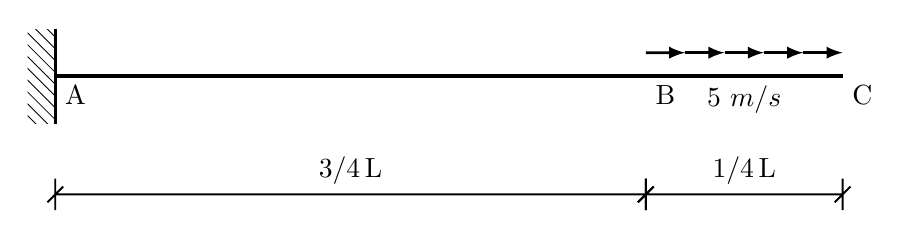
\begin{tikzpicture} 
  \scaling{2}; 
  % Nodos 
  \point{a}{0}{1};
  \point{b}{3.75}{1};
  \point{c}{5}{1};
  % Barras
  \beam{2}{a}{b};
  \beam{2}{b}{c};
  % Apoyos
  \support{3}{a}[270];
  % Fuerzas
  \lineload{4}{b}{c}[1][0.2];
  \notation{5}{b}{c}[$5\ m/s$][.5][below][2];
  % Nombres de nodos
  \notation{1}{a}{A}[below right];
  \notation{1}{b}{B}[below right];
  \notation{1}{c}{C}[below right];
  % Cotas
  \dimensioning{1}{a}{b}{0.5}[{\unit[3/4]{L}}];
  \dimensioning{1}{b}{c}{0.5}[{\unit[1/4]{L}}];
\end{tikzpicture}
}
  \caption{Geometrical description of the Dyka \cite{Dyka1995} bar.}
  \label{fig:Dyka_Bar}
\end{figure}
%%%%%%%%%%%%%%%%%%%%%%%%%%%%%%%%%%%%%%%%%%%%%%%%%%%%%%%%%%%%%%%%%%%%%%%%%%
In the proposed example, the simulation extends from time zero up to 0.00001 s.
This time interval allows the elastic wave to travel a distance of 2.6
lengths of the bar. For the spatial
discretisation, a set of seven nodal mesh sizes (0.1, 0.3325, 0.5,
1.0, 3.3325, 6.665, 10.0 millimeters) are considered. For each element a number of
four particles was selected. In the initial layout, particles are located the exact quadrature points of a linear quadrilateral, with
the exception of the \acrshort{ugimp} simulation, where gaps or overlap between
voxels of each particle are not allowed. In those cases, each particle
occupies the center of each cell quarter. For all simulations, time step
is controlled by a Courant-Friedrichs-Levy condition of 0.1, were the adopted
celerity is computed as:
\begin{equation}
  \label{eq:Cel}
  Cel = \max\{\max_{p \in \Omega_p}\{ \vec{v}_p \} , \max_{p \in \Omega_p}\{ \sqrt{\frac{E_p}{\rho_p}} \} \}.
\end{equation}
An important consideration regarding modellization concerns the
background mesh. Notice that free border of the bar has a maximum
horizontal displacement of 0.03 millimeters, therefore 
a computational domain with an extra gap of 0.03 millimeters is
required in order to accommodate the unconstrained displacement of the
particles in the left border of the bar. Naturally this problem arises
when the mesh size is small enough that relative displacement of the
particles is larger then the distance to the border, so grid crossing
phenomena could appear even in those cases with infinitesimal
displacements.

In this case, an analytical solution can be obtained
through the characteristics method, described in the appendix
\ref{app:analytical_sol}. To measure the convergence of the solutions
for the different time integration and approximation schemes the
root-mean-square (RMS) error in the velocity field is computed. RMS
error is defined as
\begin{equation}
  \label{eq:RMS}
  RMS = \sqrt{\frac{1}{N} \sum^{N}_p \left( \vec{v}_p - \hat{\vec{v}}_p \right)^2},
\end{equation}
where $\vec{v}_p$ and $\hat{\vec{v}}_p$ are respectively the analytical and
numerical solutions evaluated in the final time step in the position
of each particle. In Fig. \ref{fig:Dyka-error-evol} the evolution of the RMS is obtained for both time integration schemes. The right figure, with the \acrshort{npc} results, shows lower values of the estimated error, denoting the higher performance of this methodology. About the spatial discretisation, the \acrshort{lme} schemes show an error comparable to the obtained with the \acrshort{ugimp}, being even lower close to the grid-crossing region.

%%%%%%%%%%%%%%%%%%%%%%%%%%%%%%%%%%%%%%%%%%%%%%%%%%%%%%%%%%%%%%%%%%%%%%%%%% 
\begin{figure*}
%\sidecaption
  \centering
  \resizebox{\hsize}{!}{
    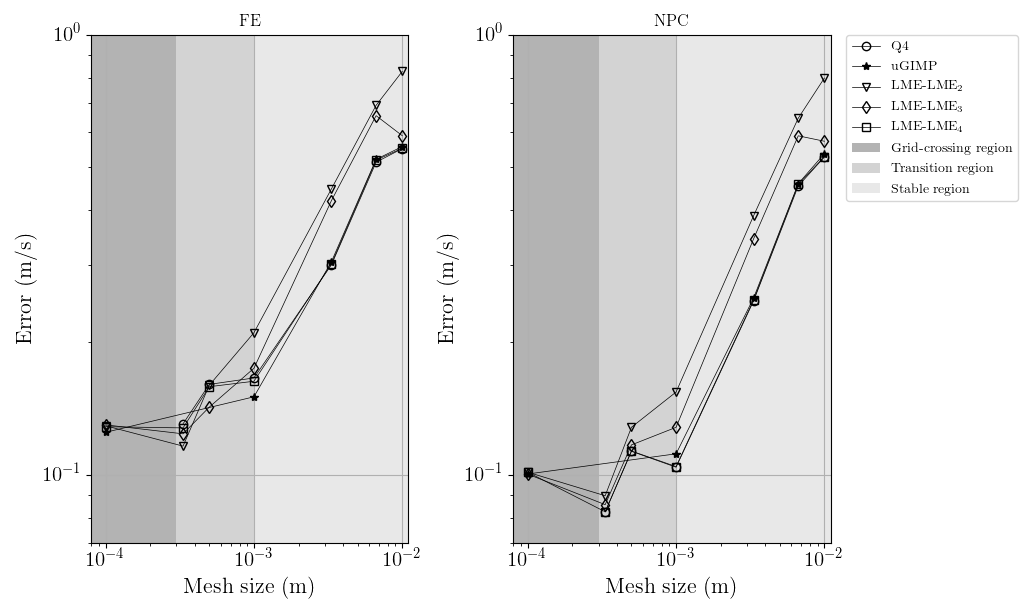
\includegraphics[width=\textwidth]{./Figures/Error_evol}
  }
  \caption{Velocity error evolution at the point A in the Dyka's bar ,
    convergence plots for \acrshort{fe} and \acrshort{npc}. The plot is subdivided with
    colours, the darker part of the diagram shows coincides when the
    relative movement of the particles is large enough to produce the
    grid crossing phenomena. The lightest part of the diagram
    coincides when the relative movement of the particles in
    negligible in comparison with the mesh size. And in the middle
    region a transition behaviour take place.}
  \label{fig:Dyka-error-evol}
\end{figure*}
%%%%%%%%%%%%%%%%%%%%%%%%%%%%%%%%%%%%%%%%%%%%%%%%%%%%%%%%%%%%%%%%%%%%%%%%%%

A first comparison between the obtained one in both time integration
schemes is plotted in figure \ref{fig:Dyka-NPC-FE}. It demonstrates the
superior performance of the \acrshort{npc} \textit{versus} the \acrshort{fe}. In the \acrshort{npc} the
spurious oscillations are quickly mitigated in the first time steps,
and the error is not propagated in time, opposite to the results of the \acrshort{fe} scheme, where the
simulation becomes unstable after $6E^{5}$ seconds.
%%%%%%%%%%%%%%%%%%%%%%%%%%%%%%%%%%%%%%%%%%%%%%%%%%%%%%%%%%%%%%%%%%%%%%%%%%
\begin{figure}
%\sidecaption
  \centering
  \resizebox{0.9\hsize}{!}{
    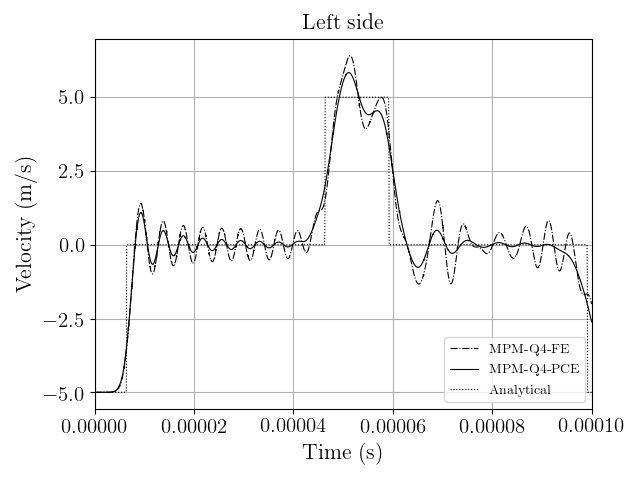
\includegraphics[width=\textwidth]{./Figures/Velocity_FE_vs_PCE_CFL_01}
  }
  \caption{Comparison of \acrshort{npc} and \acrshort{fe}
      performances: In the picture the velocity evolution at the point in the bar left side
    is plotted.}
  \label{fig:Dyka-NPC-FE}
\end{figure}
%%%%%%%%%%%%%%%%%%%%%%%%%%%%%%%%%%%%%%%%%%%%%%%%%%%%%%%%%%%%%%%%%%%%%%%%%%

Figure \eqref{fig:Dyka-LME-gamma} shows the sensitivity of the \acrshort{lme}
approximation scheme to variations in the parameter
$\gamma$, which is the one that controls the value of the regularization parameter
$\beta$ together with of the mesh size. Notice how lower values of
gamma exhibits a behaviour with a soft decay in some parts of the
simulation due to the increase of nodes adopted to regularize the
solutions. This capability could be useful in simulations where
extremely noisy oscillations could damage the solutions like memory
materials. On the other hand larger values of the parameter $\beta$
make the solution to tend to the linear \acrshort{fem} solution as the athermal limit is reached \cite{Arroyo2006}. Intermediate values of the
regularization parameters give us a compromise between both scenarios described here. An additional observation, concerning to the
solution sensibility depending on the regularization parameters, is the behaviour of the solution depending on the decreasing of mesh
size. For larger mesh sizes, where the relative particle displacement
is negligible in comparison with the cell size, the global behaviour
is \acrshort{fem}-like; therefore, larger values of $\gamma$ may offer better results. On the other hand, when mesh size is small enough to produce
grid-crossing meshfree behaviour is required to ensure the
convergence of the solution and tiny values of $\gamma$ may lead to better
performances. Convergence plot in figure \eqref{fig:Dyka-error-evol}
shows how the slope, for the larger values of $\gamma$, decreases
monotonically with the value of the mesh size, in contrast with larger
values of $\gamma$, where the performance is punished with significant
movement of the particles as far as the mesh size is reduced.
%%%%%%%%%%%%%%%%%%%%%%%%%%%%%%%%%%%%%%%%%%%%%%%%%%%%%%%%%%%%%%%%%%%%%%%%%%
\begin{figure}
%\sidecaption
  \centering
  \resizebox{0.9\hsize}{!}{
    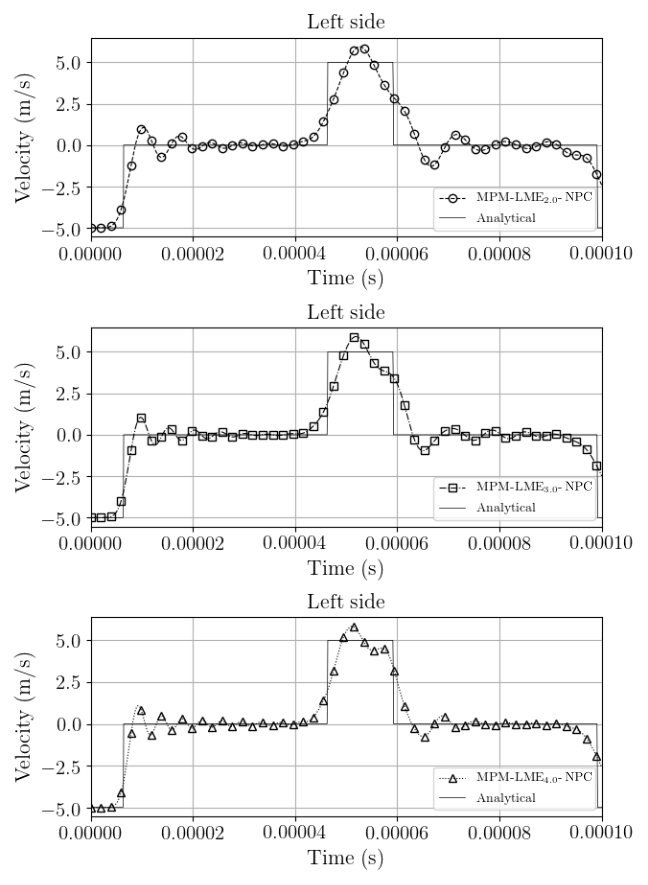
\includegraphics[width=\textwidth]{./Figures/Velocity_LME_gamma_comparative}
  }
  \caption{Sensitivity  of LME approximants performance to changes in the
    dimensionless regularization parameter $\gamma = \beta/h^2$. To
    illustrate it, the velocity evolution at the point in the bar left side
    is plotted.}
  \label{fig:Dyka-LME-gamma}
\end{figure}
%%%%%%%%%%%%%%%%%%%%%%%%%%%%%%%%%%%%%%%%%%%%%%%%%%%%%%%%%%%%%%%%%%%%%%%%%%
The performance of the
\acrshort{ugimp}~\cite{Bardenhagen2004} shape function \textit{versus} the \acrshort{lme} approximation scheme with
a dimensionless regularization parameter $\gamma$ of 4.0 is compared in Figure \ref{fig:Dyka-uGIMP-LME}. Although remarkable differences are not observed, more
robust behaviour is exhibited by the \acrshort{lme} approximants than the \acrshort{ugimp} shape functions. Regarding this, notice
the absence of \acrshort{ugimp} values for a mesh size of 0.3325 and 0.5
millimeters. The reason is due to an unstable
increasing of the error suffered during \acrshort{ugimp} simulations of these mesh sizes which yield unacceptable results. A feasible
explanation for this phenomena could be the presence of numerical
cancellation which could produce gaps between voxels. Further research
should be done in this direction for getting a better comprehension of
this phenomenon. Conversely, this shortcoming is not suffered by \acrshort{lme}, independently of regular or with irregular nodal layout.
%%%%%%%%%%%%%%%%%%%%%%%%%%%%%%%%%%%%%%%%%%%%%%%%%%%%%%%%%%%%%%%%%%%%%%%%%%
\begin{figure}
%\sidecaption
  \centering
  \resizebox{0.9\hsize}{!}{
    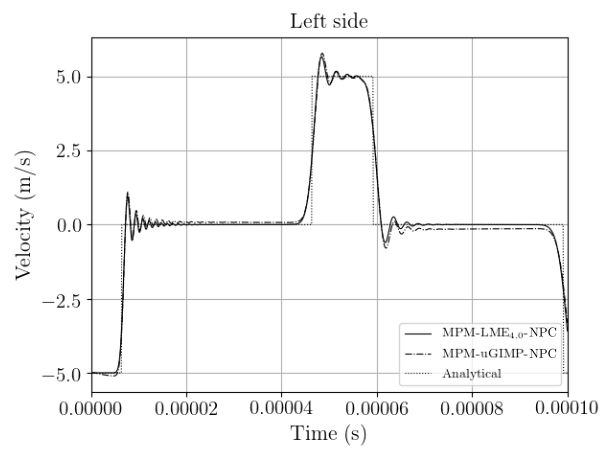
\includegraphics[width=\textwidth]{./Figures/Velocity_uGIMP_vs_LME_Dyka}
  }
  \caption{Velocity evolution at the point in the bar left side.}
  \label{fig:Dyka-uGIMP-LME}
\end{figure}
%%%%%%%%%%%%%%%%%%%%%%%%%%%%%%%%%%%%%%%%%%%%%%%%%%%%%%%%%%%%%%%%%%%%%%%%%%

Finally, the \acrshort{otm}~\cite{Li2010} solution is compared against the one obtained with \acrshort{mpm}, both with same time integration scheme and spatial discretisation, and results are shown in figure \ref{fig:Dyka-OTM-MPM}. In
this case, the performance of \acrshort{mpm} presents better robustness and stability than the
\acrshort{otm}. During the first half of the simulation both method 
seem to perform in a similar way, but during the second half of the
simulation after the elastic wave has travel from the free border to
the fixed one and back, in \acrshort{otm} the solution becomes more noisy than the
one performed by \acrshort{mpm}.  
%%%%%%%%%%%%%%%%%%%%%%%%%%%%%%%%%%%%%%%%%%%%%%%%%%%%%%%%%%%%%%%%%%%%%%%%%%
\begin{figure}
%\sidecaption
  \centering
  \resizebox{0.9\hsize}{!}{
    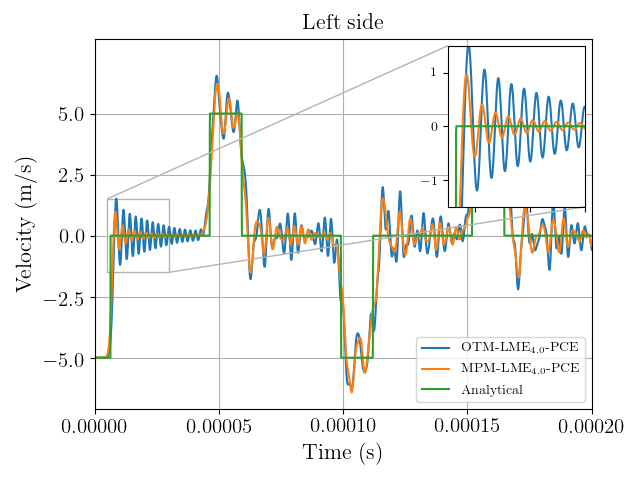
\includegraphics[width=\textwidth]{./Figures/Velocity_MPM_vs_OTM_Dyka}
  }
  \caption{Velocity evolution at the point in the bar left side.}
  \label{fig:Dyka-OTM-MPM}
\end{figure}
%%%%%%%%%%%%%%%%%%%%%%%%%%%%%%%%%%%%%%%%%%%%%%%%%%%%%%%%%%%%%%%%%%%%%%%%%%

\clearpage
\subsection{Rigid block}
\label{sec:andersen-block}

The following test was proposed to validate the ability of the proposed
interpolation technique to deal with grid crossing instabilities. It
consists of the simulation of a square block of soil incrementally
loaded by a body force. Details of the problem are sketched in figure~\ref{fig:block}
%%%%%%%%%%%%%%%%%%%%%%%%%%%%%%%%%%%%%%%%%%%%%%%%%%%%%%%%%%%%%%%%%%%%%%%%%%
\begin{figure}
%\sidecaption
  \centering
  \resizebox{0.7\hsize}{!}{
    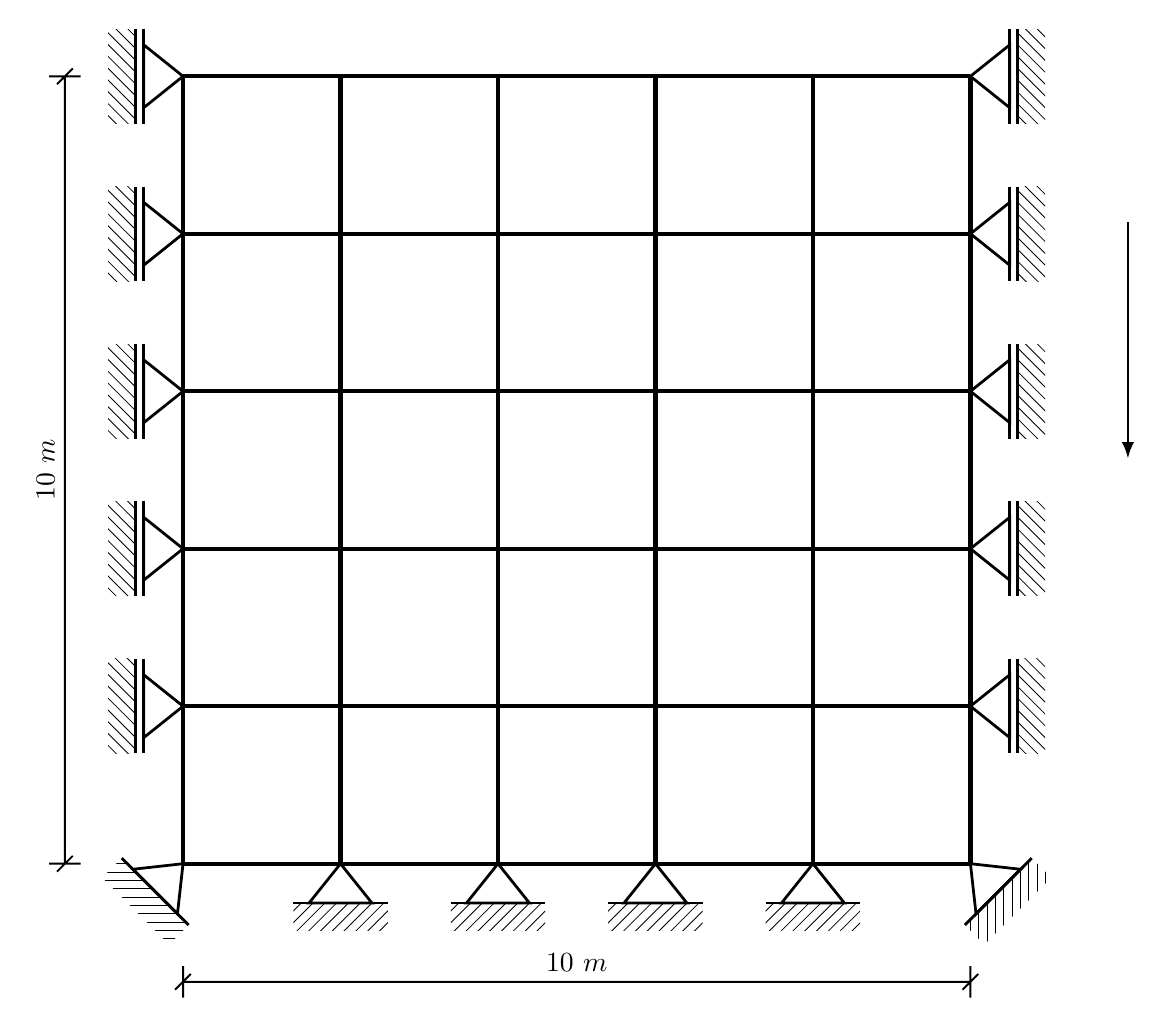
\begin{tikzpicture} 
  \scaling{1};
  
% Nodos
\point{1}{0}{10};
\point{2}{2}{10};
\point{3}{0}{8};
\point{4}{2}{8};
\point{5}{4}{10};
\point{6}{0}{6};
\point{7}{2}{6};
\point{8}{4}{8};
\point{9}{4}{6};
\point{10}{6}{10};
\point{11}{0}{4};            
\point{12}{2}{4};            
\point{13}{6}{8};            
\point{14}{4}{4};            
\point{15}{6}{6};            
\point{16}{8}{10};            
\point{17}{0}{2};            
\point{18}{2}{2};            
\point{19}{8}{8};            
\point{20}{6}{4};            
\point{21}{4}{2};            
\point{22}{8}{6};            
\point{23}{0}{0};            
\point{24}{10}{10};            
\point{25}{6}{2};            
\point{26}{8}{4};
\point{27}{2}{0};            
\point{28}{10}{8};            
\point{29}{4}{0};            
\point{30}{10}{6};            
\point{31}{8}{2};            
\point{32}{6}{0};            
\point{33}{10}{4};            
\point{34}{8}{0};            
\point{35}{10}{2};            
\point{36}{10}{0};

% Barras
\beam{2}{27}{18};
\beam{2}{18}{17};
\beam{2}{17}{23};
\beam{2}{23}{27};
  
\beam{2}{29}{21};
\beam{2}{21}{18};
\beam{2}{18}{27};
\beam{2}{29}{27};

\beam{2}{32}{25};
\beam{2}{25}{21};
\beam{2}{21}{29};
\beam{2}{32}{29};

\beam{2}{34}{31};
\beam{2}{31}{25};
\beam{2}{25}{32};
\beam{2}{34}{32};

\beam{2}{36}{35};
\beam{2}{35}{31};
\beam{2}{31}{34};
\beam{2}{36}{34};

%%%%%%%%%%%%%%%%
\beam{2}{18}{12};
\beam{2}{12}{11};
\beam{2}{11}{17};
\beam{2}{18}{17};

\beam{2}{21}{14};
\beam{2}{14}{12};
\beam{2}{12}{18};
\beam{2}{21}{18};

\beam{2}{25}{20};
\beam{2}{20}{14};
\beam{2}{14}{21};
\beam{2}{25}{21};

\beam{2}{31}{26};
\beam{2}{26}{20};
\beam{2}{20}{25};
\beam{2}{31}{25};

\beam{2}{35}{33};
\beam{2}{33}{26};
\beam{2}{26}{31};
\beam{2}{35}{31};

%%%%%%%%%%%%%%%%
\beam{2}{12}{7};
\beam{2}{7}{6};
\beam{2}{6}{11};
\beam{2}{12}{11};

\beam{2}{14}{9};
\beam{2}{9}{7};
\beam{2}{7}{12};
\beam{2}{14}{12};

\beam{2}{20}{15};
\beam{2}{15}{9};
\beam{2}{9}{14};
\beam{2}{20}{14};

\beam{2}{26}{22};
\beam{2}{22}{15};
\beam{2}{15}{20};
\beam{2}{26}{20};

\beam{2}{33}{30};
\beam{2}{30}{22};
\beam{2}{22}{26};
\beam{2}{33}{26};

%%%%%%%%%%%%%%%%
\beam{2}{7}{4};
\beam{2}{4}{3};
\beam{2}{3}{6};
\beam{2}{7}{6};

\beam{2}{9}{8};
\beam{2}{8}{4};
\beam{2}{4}{7};
\beam{2}{9}{7};

\beam{2}{15}{13};
\beam{2}{13}{8};
\beam{2}{8}{9};
\beam{2}{15}{9};

\beam{2}{22}{19};
\beam{2}{19}{13};
\beam{2}{13}{15};
\beam{2}{22}{15};

\beam{2}{30}{28};
\beam{2}{28}{19};
\beam{2}{19}{22};
\beam{2}{30}{22};

%%%%%%%%%%%%%%%%
\beam{2}{4}{2};
\beam{2}{2}{1};
\beam{2}{1}{3};
\beam{2}{4}{3};

\beam{2}{8}{5};
\beam{2}{5}{2};
\beam{2}{2}{4};
\beam{2}{8}{4};

\beam{2}{13}{10};
\beam{2}{10}{5};
\beam{2}{5}{8};
\beam{2}{13}{8};

\beam{2}{19}{16};
\beam{2}{16}{10};
\beam{2}{10}{13};
\beam{2}{19}{13};

\beam{2}{28}{24};
\beam{2}{24}{16};
\beam{2}{16}{19};
\beam{2}{28}{19};

% Bottom
\support {1}{23}[315];
\support {1}{27}[0];
\support {1}{29}[0];
\support {1}{32}[0];
\support {1}{34}[0];
\support {1}{36}[45];

% \support {2}{23}[270];
\support {2}{1}[270];
\support {2}{3}[270];
\support {2}{6}[270];
\support {2}{11}[270];
\support {2}{17}[270];

\support {2}{24}[90];
\support {2}{28}[90];
\support {2}{30}[90];
\support {2}{33}[90];
\support {2}{35}[90];
% \support {2}{36}[90];

% Gravity
\point{g}{12}{5};
\load{1}{g}[90][3][0];

% Cotas
\dimensioning{1}{23}{36}{-1.5}[$10~m$];
\dimensioning{2}{23}{1}{-1.5}[$10~m$];


\end{tikzpicture}


% % Apoyos
% \support{3}{c}[90];
% % Fuerzas
% \lineload{4}{b}{a}[1][0.2];
% \notation{5}{a}{b}[$-5\ m/s$][.5][below][2];
% % Nombres de nodos
% \notation{1}{a}{A}[below left];
% \notation{1}{b}{B}[below left];
% \notation{1}{c}{C}[below left];
% % Cotas
% \dimensioning{1}{a}{b}{0.5}[{\unit[1/4]{L}}];
% \dimensioning{1}{b}{c}{0.5}[{\unit[3/4]{L}}];


% End Elements
}
  \caption{Geometrical description of a soil block }.
  \label{fig:block}
\end{figure}
%%%%%%%%%%%%%%%%%%%%%%%%%%%%%%%%%%%%%%%%%%%%%%%%%%%%%%%%%%%%%%%%%%%%%%%%%%
This test was previously proposed by Andersen (2009)\cite{thesis_Andersen_2009}. The
elastic parameters considered for this test are: 
\begin{itemize} 
\item  Initial density : $6\cdot 10^3\ kg/m^3$
\item  Poisson ratio : $0$
\item  Elastic modulus : $5\ MPa$
\end{itemize}
The gravity force is applied as an external force. Using a total time period of T (20
seconds) to apply the gravity, it is increased from 0 to 9.81$m/s$
with a sinusoidal function until T/2 and then maintained constant until T
in order to reach the equilibrium state:
\begin{equation}
  \label{eq:gravity-load-block}
 \mathbf{g}(t) = \left\{
    \begin{array}{ll}
      0.5 \mathbf{g} (\sin(\frac{2t \pi}{T} - \frac{\pi}{2})+1)  & \mbox{if } t \leq T/2 \\
      \mathbf{g} & \mbox{if } t > T/2
    \end{array}
  \right.
\end{equation}
In order to get a stable solution, time step was conducted by a
Courant number of 0.1. On the other hand, the explicit
predictor-corrector scheme is here employed looking forward to getting better results. For the
initial spatial discretisation four particles per cell
($\Delta x = 2\ m$) were adopted. The initial layout of particles inside of the
cell changes according to the approximation technique adopted. For the
bi-linear shape functions and the \acrshort{lme} approximants, the initial
position corresponds to the location of the gauss-points in a standard
quadratic finite element. For the \acrshort{ugimp} shape function the initial
position of each particle is located in the center of each voxel, due
to the fact that in the initial situation, the voxel domain should not
overlap each others.

Figure~\ref{fig:Block-LME3} shows the evolution of the vertical stress
during the loading process. The result is physically realistic as
the stress increases linearly from the top to the bottom of the specimen,
and the value of the vertical stress in a material point located in
the bottom of the specimen oscillates around $5.2 MPa$, which is
the analytic value given by $\sigma_{yy} = \rho g h_y$.
%%%%%%%%%%%%%%%%%%%%%%%%%%%%%%%%%%%%%%%%%%%%%%%%%%%%%%%%%%%%%%%%%%%%%%%%%%
\begin{figure*}
  \centering
  \subfigure[t = 0 seconds.]{
    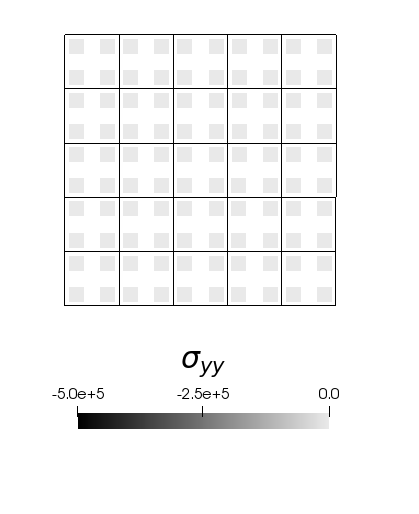
\includegraphics[width=0.3\textwidth]{Figures/Block_LME3_PCE_a_t0}
  }
  \subfigure[t = 5 seconds.]{
    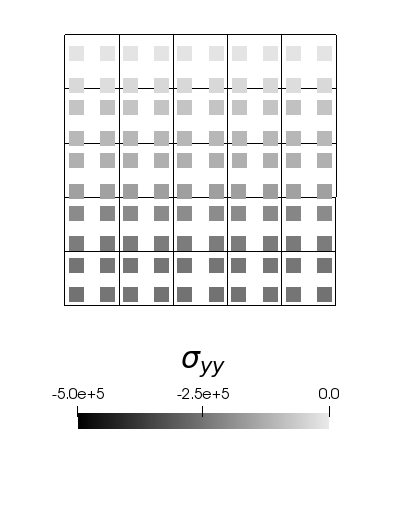
\includegraphics[width=0.3\textwidth]{Figures/Block_LME3_PCE_b_t025}
  }
  \subfigure[t = 20 seconds]{
    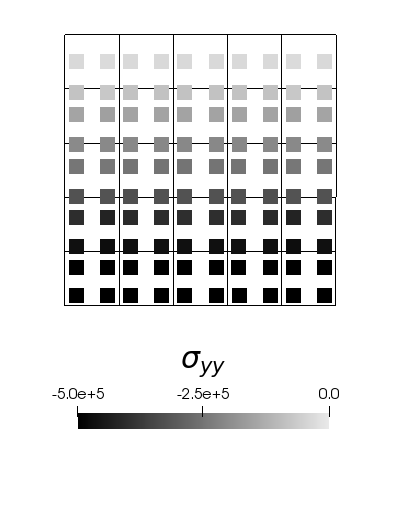
\includegraphics[width=0.3\textwidth]{Figures/Block_LME3_PCE_c_t1}
  }
  \caption{Vertical normal stress and position of material points
    during the loading process for a soft soil ($E = 5\ MPa$, $\rho_0
    = 6\cdot 10^3\ kg/m^3$). Numerical parameters considered for the
    simulation are : Local \textit{max-ent} shape function $\gamma =3$
    and explicit PC scheme with CFL 0.1.}
  \label{fig:Block-LME3}
\end{figure*}
%%%%%%%%%%%%%%%%%%%%%%%%%%%%%%%%%%%%%%%%%%%%%%%%%%%%%%%%%%%%%%%%%%%%%%%%%%

Figure~\ref{fig:vertical-displacement-block} shows the vertical
displacement evolution of a point in the free surface of the
block. This figure shows how simulations performed with a bi-linear
interpolation technique (Q4) turns out to be unstable during
cell-crossing and consequently fail. The \acrshort{ugimp} simulation
is more stable than the one performed by the Q4, although is still
unstable and could trigger severe oscillations in simulation with
non-linear  materials. The \acrshort{lme} simulation was performed
using two kinds of shape functions, one with a low value of the
dimensionless parameter, $\gamma = 0.8$, and other with a larger value
of it, $\gamma = 3.0$. Notice that the results are both stable, but
the larger values of $\gamma$ give us a very stable solution. This is
due to the fact that with larger value of $\gamma$, the shape
functions behaves in a similar way to the \acrshort{fem}, which performs very
accurate in those cases with a reasonable mesh distorsion, and with a
lower value it behaves in a similar way to the \acrshort{ugimp}. This behaviour
was noticed previously by \cite{Arroyo2006}, were authors highlighted
how, by adjusting the spatial variation of $\beta(\vec{x})$, it is
possible to select regions of the domain of analysis which are treated
by finite elements and regions that are treated in the style of
meshfree methods, with seamless transitions between those regions. 
%%%%%%%%%%%%%%%%%%%%%%%%%%%%%%%%%%%%%%%%%%%%%%%%%%%%%%%%%%%%%%%%%%%%%%%%%%
\begin{figure}
%\sidecaption
  \centering
  \resizebox{\hsize}{!}{
    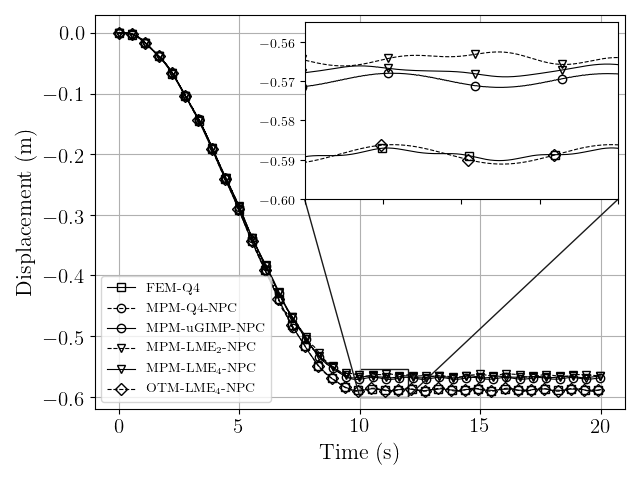
\includegraphics[width=\textwidth]{./Figures/Block_CFL_01_Comparative}
  }
  \caption{Comparative of the vertical displacement evolution in a
    point located in the free surface employing different
    interpolation schemes and numerical techniques.} 
  \label{fig:vertical-displacement-block}
\end{figure}
%%%%%%%%%%%%%%%%%%%%%%%%%%%%%%%%%%%%%%%%%%%%%%%%%%%%%%%%%%%%%%%%%%%%%%%%%%

\MODIFIED{\subsection{Velocity waves in an elastic domain}}
\label{sec:Velocity-waves-elastic-domain}

\MODIFIED{The following test is best suited to validate the ability of the discussed
time integration scheme to reproduce 2D wave propagation problem.  It consists of the side impact of a moving elastic square. The square was 50 x 50 m and modeled with the following elastic parameters :
\begin{itemize} 
\item  Initial density : $20 kg/m^3$
\item  Poisson ratio : $0.3$
\item  Elastic modulus : $0.1 MPa$
\end{itemize}
}

\MODIFIED{The background set of nodes consists in a cartesian grid with a uniform gap between nodes of 1 mm, and square was discretised with four material points by cell. The courant number is fixed to 0.1 during the whole simulation and $\text{LME}_{4.0}$ shape functions where used. The square initially move horizontally through the grid at $\text{V}_0 = 1.0 m/s$ until it hits an obstacle modelled as a set of nodes with  zero velocity prescribed. The collision produce stress waves and cause the square to bounce back.}

\MODIFIED{Snapshots of velocity field magnitude within the square are given in\ref{fig:Magnitude_velocity_impact_square}. At early times, \acrshort{npc} and \acrshort{fe} are similar. At later times, the \acrshort{fe} introduces significant numerical noise while \acrshort{npc} is almost clean. }
%%%%%%%%%%%%%%%%
\begin{figure}
%\sidecaption
  \centering
  \resizebox{\hsize}{!}{
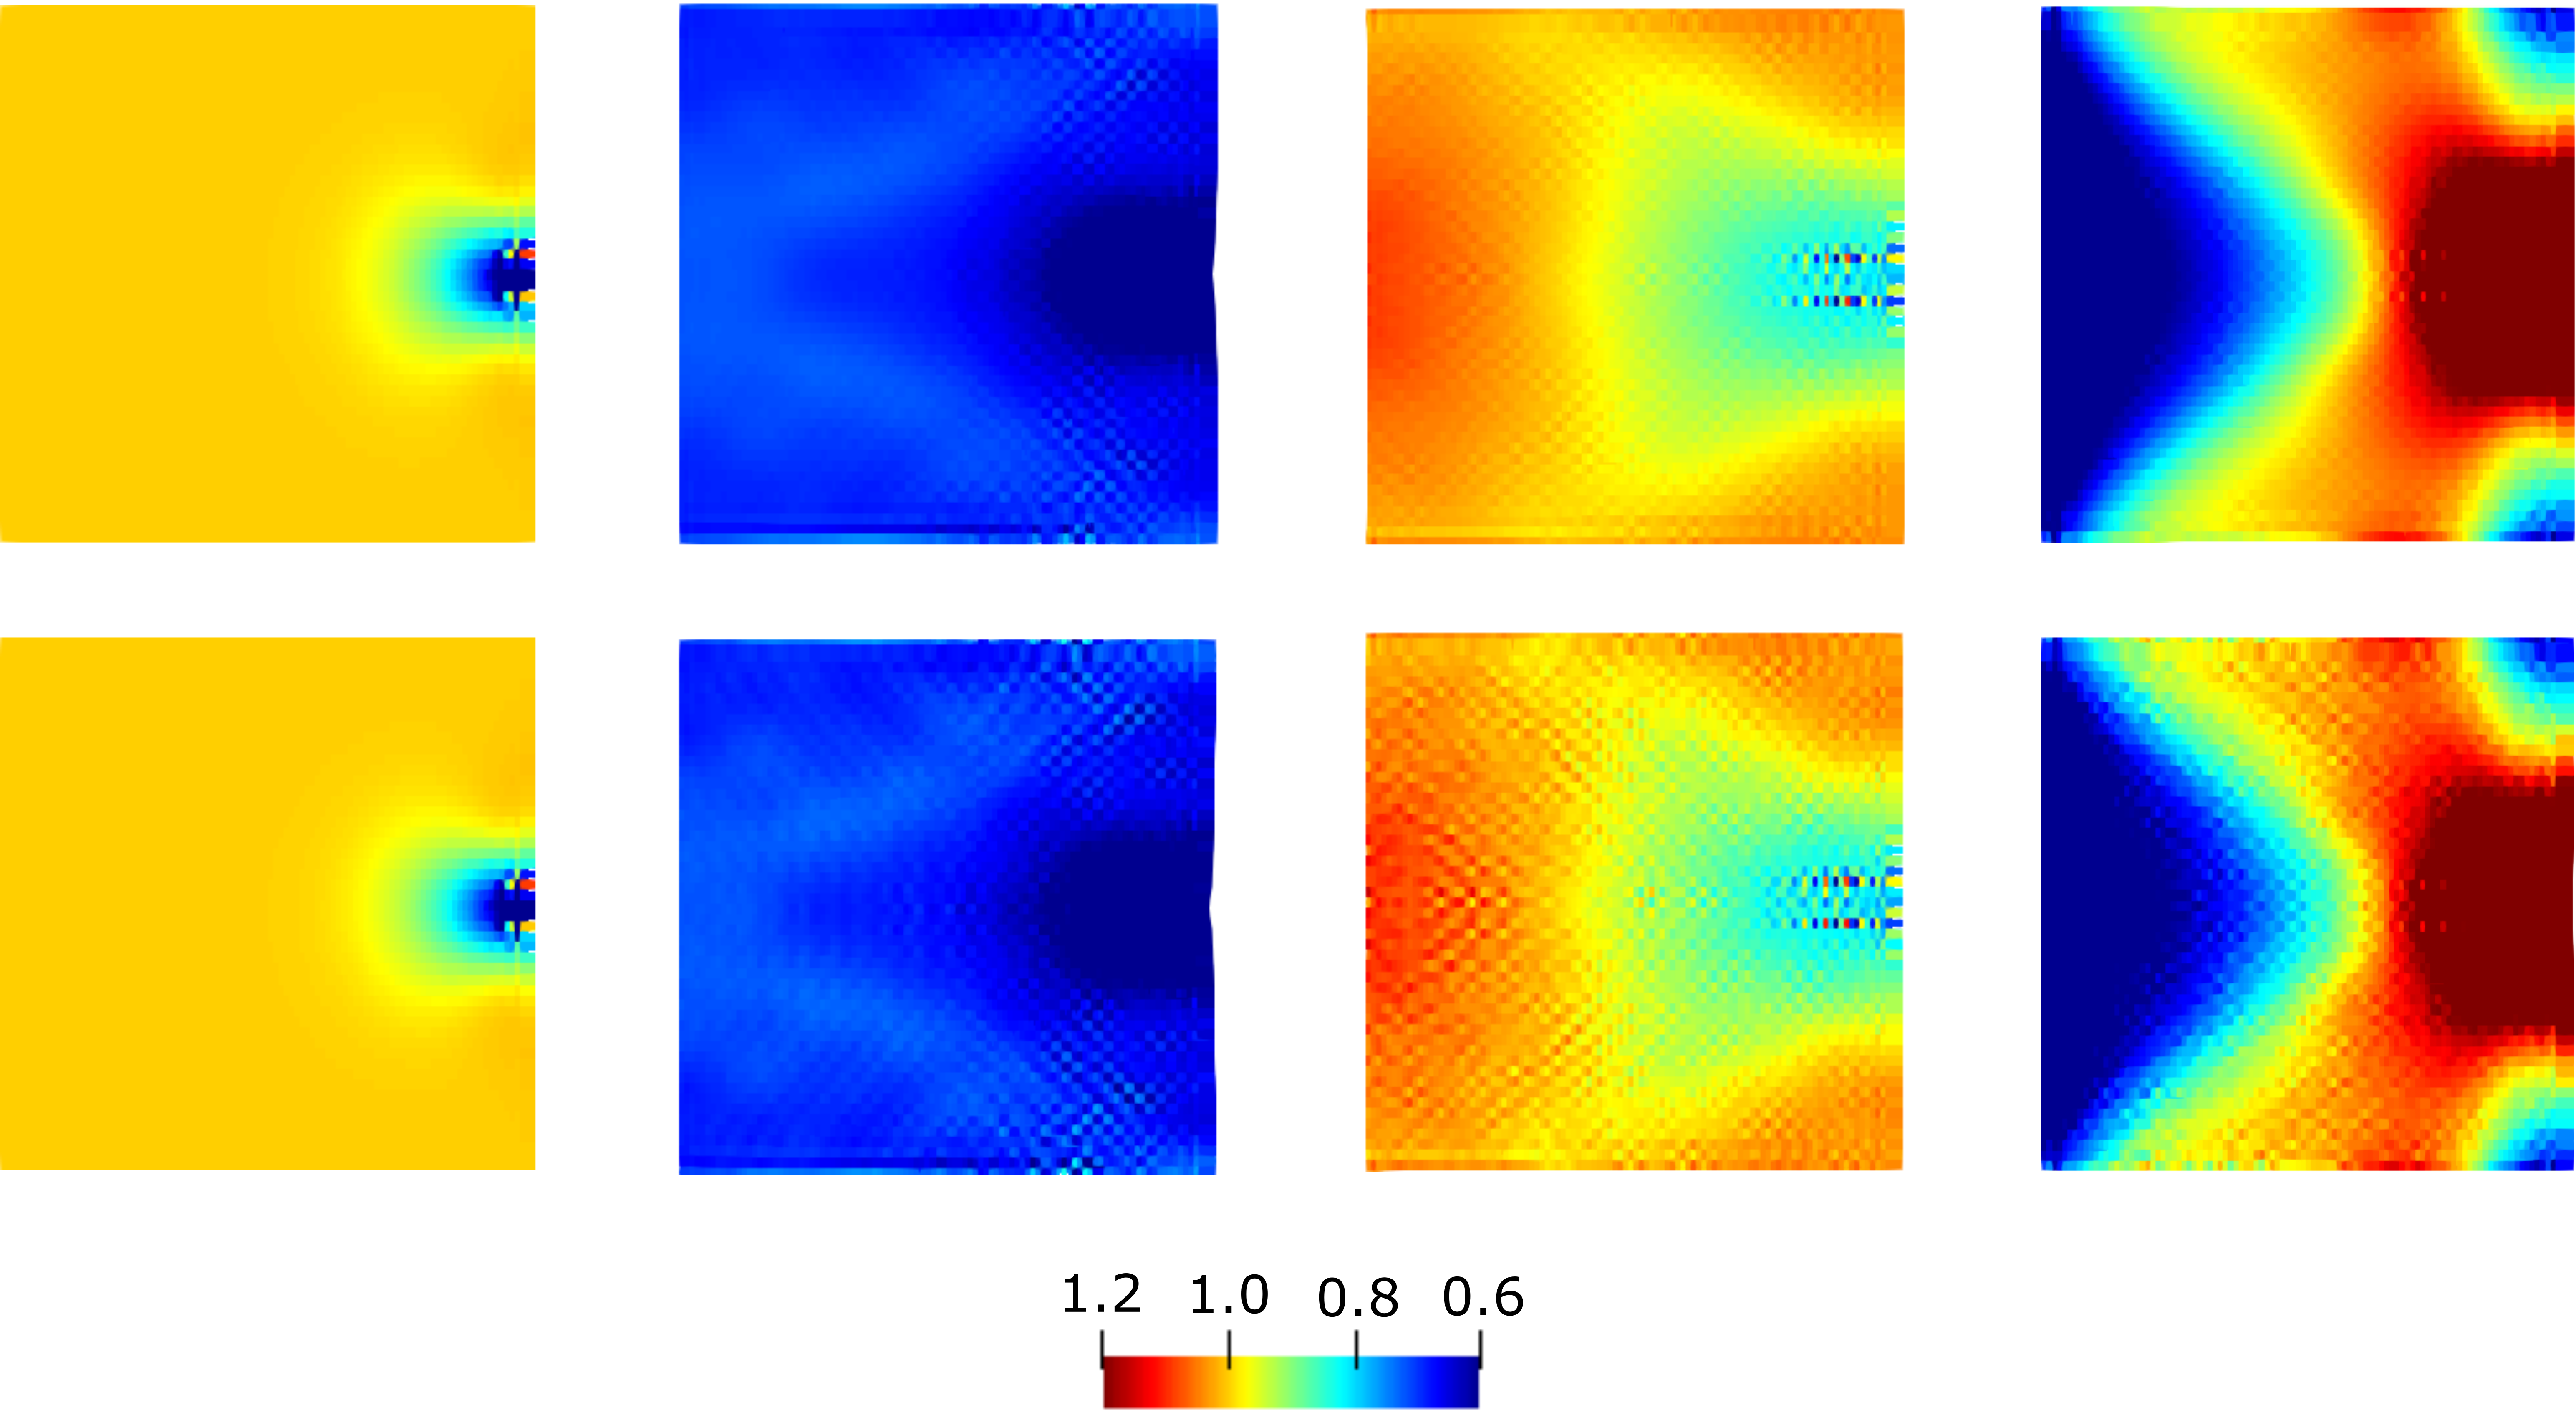
\includegraphics[scale=1]{Figures/Velocity_FE_vs_NPC_square.png} 
  }
  \caption{Snapshots of velocity magnitudes in an elastic square impacted at a point on the right edge. The top row is for \acrshort{npc} updates and the bottom row is for \acrshort{fe} updates.}
  \label{fig:Magnitude_velocity_impact_square}
\end{figure}
%%%%%%%%%%%%%%%% 
\MODIFIED{Energy plots in figure \ref{fig:Energy_impact_square} shows that after collision the total amount of energy is preserved. In the bounce back stress wave are still travelling thorough the elastic domain introducing numerical noise due to the inaccuracies of the time integration scheme as figure \ref{fig:Magnitude_velocity_impact_square} proves. However, \acrshort{npc} introduces a minimal energy loss (less than 0.1\%) to significantly reduce the numerical noise. }

\MODIFIED{Although during impact mechanical energy decreases, no real dissipation occurs since after collision the value is again 25 kJ like before collision. Furthermore, kinetic energy has been exactly computed. Hence, this apparently dissipation of mechanical energy is probably due to numerical cancellation of shear terms contribution. }
%%%%%%%%%%%%%%%%
\begin{figure}
%\sidecaption
  \centering
  \resizebox{0.8\hsize}{!}{
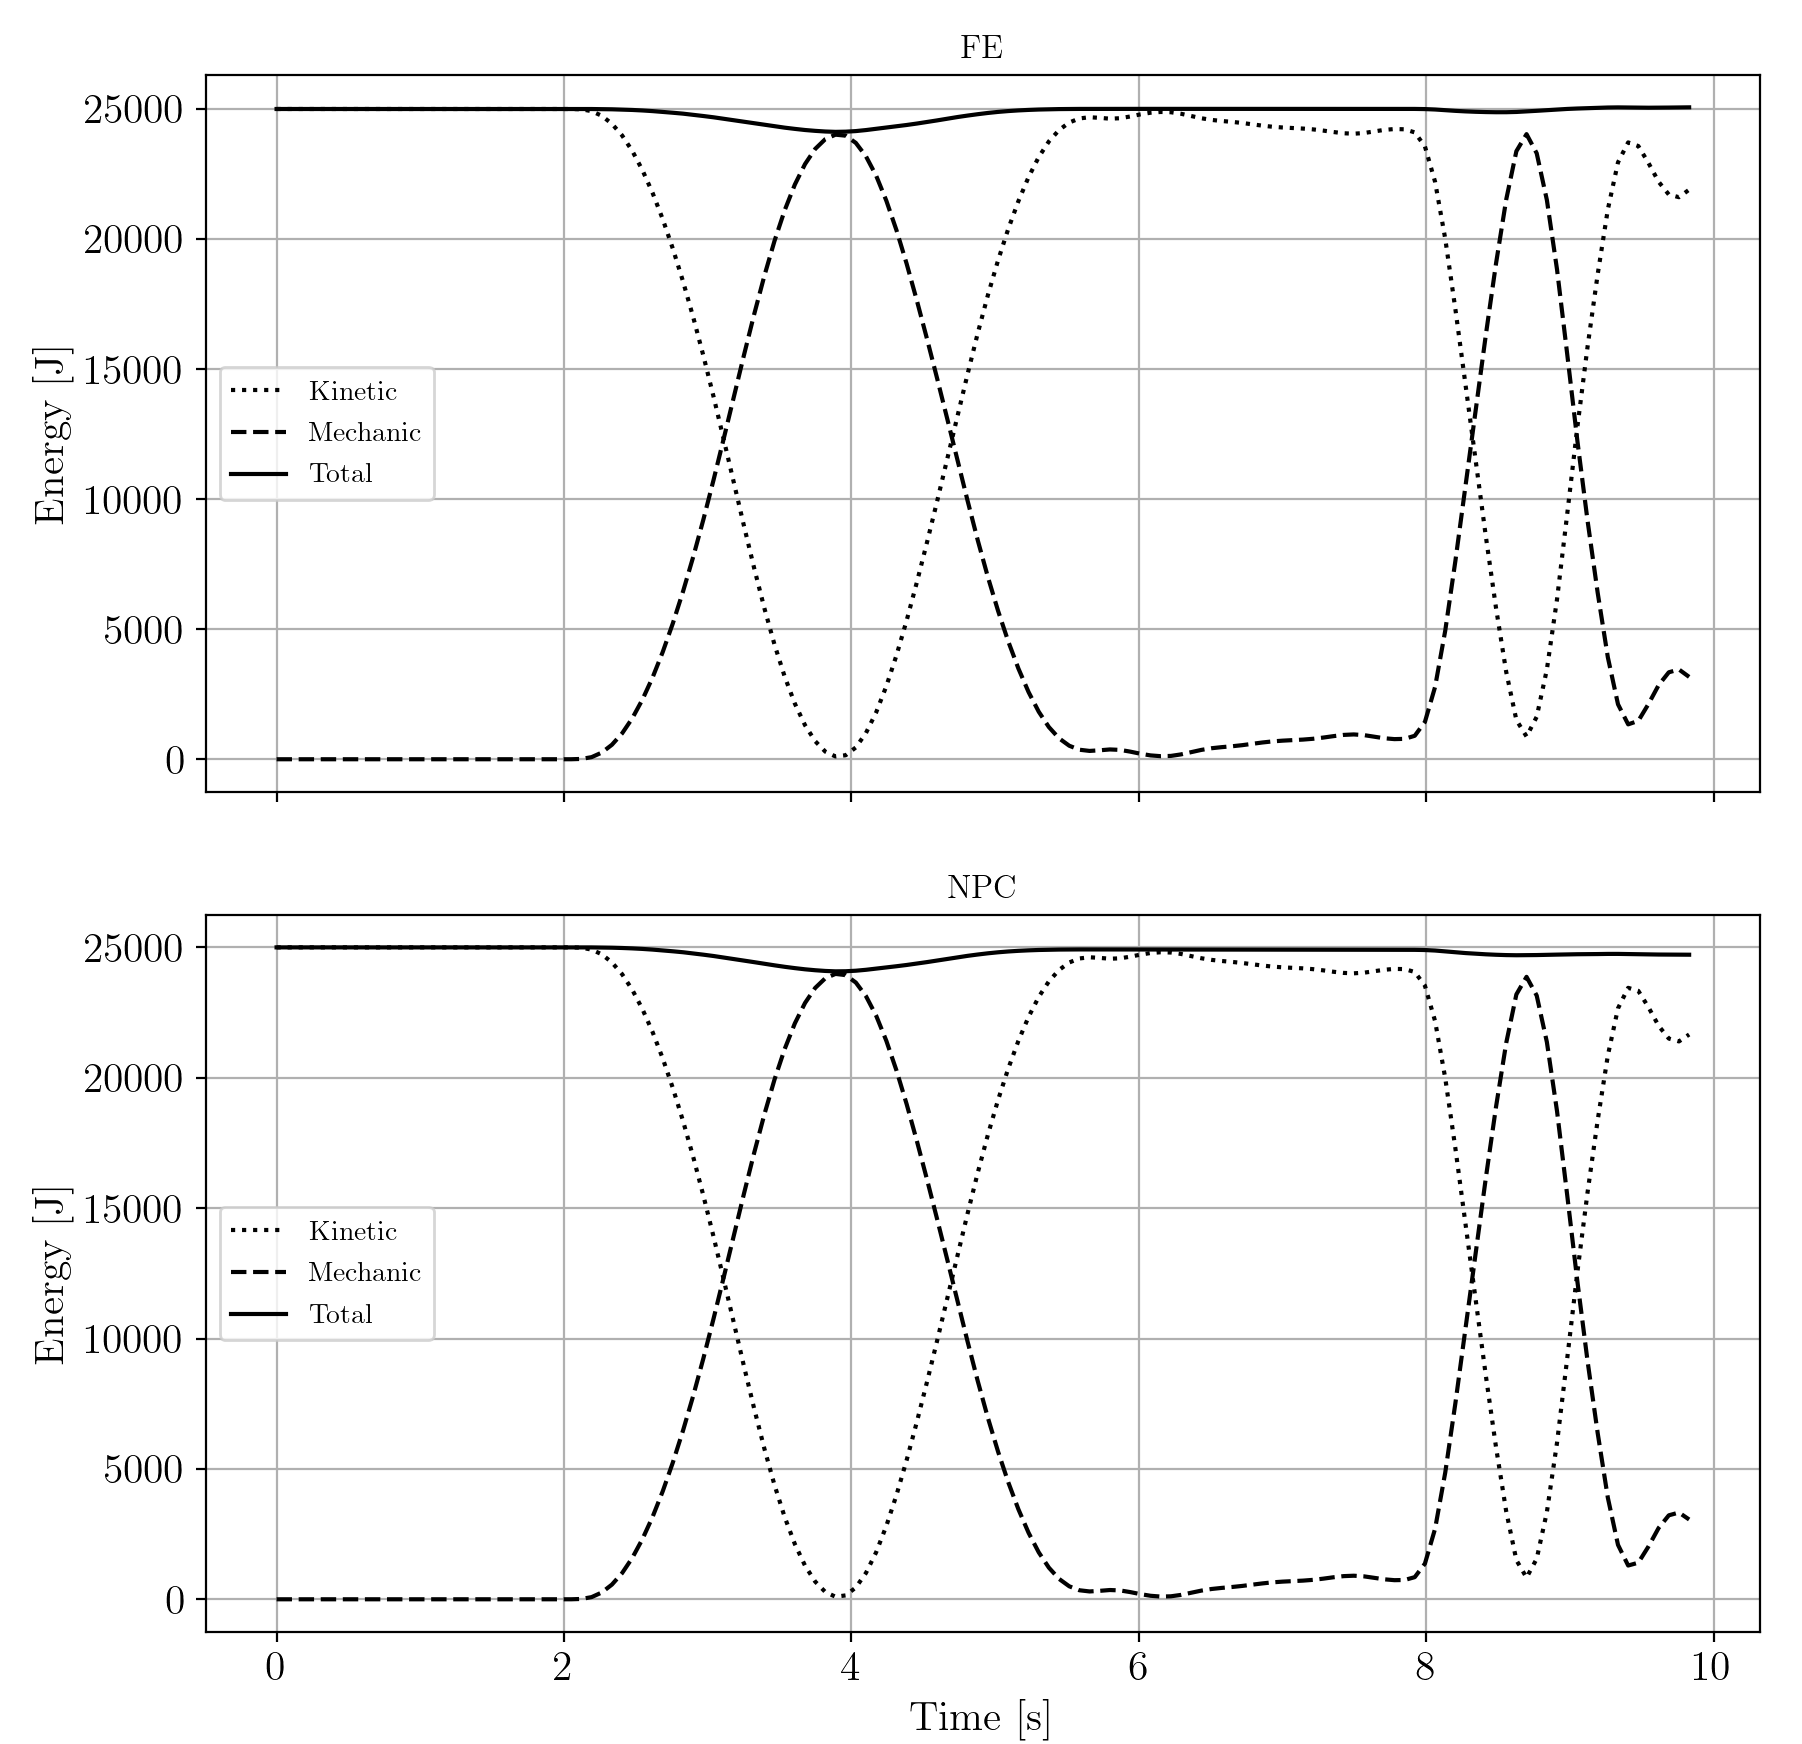
\includegraphics[scale=1]{Figures/Energy_square.png} 
  }
  \caption{Total energy (kinetic energy plus strain energy) evolution for the square. Solid line represent total energy, dashed line represent strain energy, and dotted line represent kinetic energy.}
  \label{fig:Energy_impact_square}
\end{figure}
%%%%%%%%%%%%%%%% 

\section{Conclusions}
\label{sec:conclusions}
We have proposed in this paper an enhanced methodology which improves \acrfull{mpm} behaviour in fast dynamics problems. Different time and space discretisation techniques have been presented and their performance being compared agains other approaches in two benchmark problems.
First, a novel time integration scheme for \acrshort{mpm} has been carried out. The \acrshort{npc} has been shown to be a highly efficient alternative for demanding fast dynamics problems. In the literature, several approaches of the \acrshort{npc} are proposed in order to compete on accuracy with expensive implicit time integration algorithms. The main achievement of the proposed time discretisation has been observed within the Dyka's bar \ref{sec:dyka-bar}, obtaining lower values of the error than the ones obtained with the \acrfull{fe} scheme, \MODIFIED{with a minimal loose of energy as in highlighted in \ref{sec:Velocity-waves-elastic-domain} }.
Also, the procedure employed to design the \acrshort{npc} algorithm opens the
door to revisit a huge variety of time integration schemes developed
originally for \acrshort{fem}, which can be implemented within a \acrshort{mpm} framework with the suitable modifications. In addition to the implementation of enhanced time integration schemes, further research can be done in the analysis of the good performance of the algorithm within non-linear solutions, such as the coupling between different phases or the non-linear constitutive behaviour of the materials: the employment of this scheme to strengthen the localization capabilities of \acrshort{mpm} for viscoplastic materials is on the scope of this research line. The comparison with traditional time schemes in the non-linear field will improve the formal understanding of the proposed methodology.

On the other hand, the spatial discretisation of the \acrshort{mpm} is enhanced thanks to the powerful skills of the \acrfull{lme} approximation scheme, which has been validated as a robust and versatile
tool in the \acrshort{mpm} framework. It also comes up as a promising
alternative to other approximation techniques, developed within the
\acrshort{mpm} framework, in order to overcome grid crossing limitations and to avoid the
constriction of the \acrshort{ugimp} of a regular mesh or a high
density of particles per cell. Several research lines of the \acrshort{lme} scheme dive into the improvement of the methodology, focusing in the optimization of the calculation of the shape function and the possibility of adapting the parameter $\beta(\vec{x})$ through the finite strain
tensor in order to align the shape functions in the principal strain
direction to select the most suitable set of nodes adapted to the strain as well as the possibility of adapting the value of $\beta$ to solve the equations
\acrshort{fem}-like of meshfree-like depending of how behaves the
region. Together with the implementation of non-linear behaviours, previously mentioned, challenging
scenarios could be reproduced, being the main purpose of the research line the simultaneous simulation of both initialization and
propagation stages of fast landslides.

% 
\section*{Conflict of interest}
%
The authors declare that they have no conflict of interest.

% 
\section*{Acknowledgements}
%
The financial support to develop this research from the Ministerio de Ciencia e Innovaci\'on, under Grant No. BIA-2016-76253 is greatly appreciated. The first and the second authors also acknowledge the fellowship Fundaci\'on Agust\'in de Betancourt and Juan de la Cierva (FJCI-2017–31544) respectively.


% \printglossary[type=\acronymtype]
\printglossaries

\appendix

\section{The analytical solution of the 1D Dyka benchmark}
\label{app:analytical_sol}

For the derivation of this analytical solution, a 1D elastic bar is
consider. Henceforth for convenience the governing equations will be written in terms of stress and velocity. The balance of linear momentum,
\begin{equation}
  \label{eq:1D-balance-linear-momentum}
  \rho\ \Deriv{v}{t} = \Deriv{\sigma}{x},
\end{equation}
Secondly the constitutive equation is the well known linear
elastic one,
\begin{equation}
  \label{eq:1D-constitutive-equation}
  \Deriv{\sigma}{t} = E \Deriv{\varepsilon}{t},
\end{equation}
where $E$ is the elastic modulus. And finally the compatibility
equation,
\begin{equation}
  \label{eq:CompatibilityEquation_e}
  \Deriv{\varepsilon}{t} = \Deriv{v}{x}.
\end{equation}
Next for simplicity, we will introduce
\eqref{eq:CompatibilityEquation_e} in
\eqref{eq:1D-constitutive-equation}, it yield to,
\begin{align}
  \label{eq:1D-balance-linear-momentum-II}
  \Deriv{v}{t} &= \frac{1}{\rho}\ \Deriv{\sigma}{x}, \\
  \label{eq:1D-constitutive-equation-II}
  \Deriv{\sigma}{t} &= E\ \Deriv{v}{x}.
\end{align}
Introducing \eqref{eq:1D-constitutive-equation-II} in
\eqref{eq:1D-balance-linear-momentum-II} and expressing the remaining equation in terms of the displacement, results the wave equation for linear elastic materials,
\begin{equation}
  \label{eq:1D-wave-elastic}
  \Deriv[2]{u}{t} = \frac{E}{\rho}\ \Deriv[2]{u}{x} = c^2\ \Deriv[2]{u}{x}
\end{equation}
where $c = \sqrt{\frac{E}{\rho}}$ is the material celerity. Alternative, rearranging both equations \eqref{eq:1D-balance-linear-momentum-II} and
\eqref{eq:1D-constitutive-equation-II} it is possible to join them in a single system of equations as,
\begin{equation}
  \label{eq:System-stress-velocity}
  \Deriv{}{t} \left[
    \begin{array}{c}
      \sigma \\
      v
    \end{array}
  \right] + \left[
    \begin{array}{cc}
      0 & - E \\
      - 1/\rho & 0 
    \end{array} \right] \left[
    \begin{array}{c}
      \Deriv{\sigma}{x} \\
      \Deriv{v}{x}
    \end{array}
  \right] = \Vector{0}.
\end{equation}
Or in a more compact format,
\begin{equation}
  \label{eq:System-stress-velocity-II}
  \Deriv{\Vector{\phi}}{t} + \Matrix{A}\Deriv{\Vector{\phi}}{x} = \Vector{0}.
\end{equation}
In \eqref{eq:System-stress-velocity-II} stress and velocity are joined in to a single structure $\Vector{\phi}$ and $\Matrix{A}$ in coupling matrix between both equations,
\begin{equation*}
  \Vector{\phi} = \left[
    \begin{array}{c}
      \sigma \\
      v
    \end{array}
  \right],\quad 
  \Matrix{A} =  \left[
    \begin{array}{cc}
      0 & - E\\
      - 1/\rho & 0 
    \end{array} \right].
\end{equation*}
Despite of this manipulation, the nature
of \label{eq:eq:System-stress-velocity-II} is still hyperbolic. A
proof of this can be easily obtained computing the zeros of the
hypersurface defined by \eqref{eq:1D-wave-elastic}. And later the
eigenvalues of $\Matrix{A}$ in \eqref{eq:System-stress-velocity-II}. In both cases, eigenvalues are real and distinct ($\lambda = \pm \sqrt{\frac{E}{\rho}}$),
therefore the system is called strictly hyperbolic. Assuming that  $\Matrix{A}$ has $n$ different eigenvalues $\{ \lambda_1, \ldots, \lambda_i, \ldots
\lambda_n \}$ and $n$ eigenvectors $\{ \vec{x}^1, \ldots,
\vec{x}^i, \ldots \vec{x}^n \}$ satisfying that $\tens{A} \vec{x} =
\lambda \vec{x} $. Now we introduce the matrix $\Matrix{P}$ whose columns are the $n$ eigenvalues $\Vector{x}$
\begin{equation}
  \label{eq:P-matrix}
\Matrix{P} = \{ \vec{x}^1, \vec{x}^2, \vec{x}^3, \ldots \vec{x}^n \}.
\end{equation}
Diagonalizing $\Matrix{A}$ using $\Matrix{P}$ yields,
\begin{equation}
  \label{eq:Lambda-matrix}
  \Lambda = \Matrix{P}^{-1} \Matrix{A}\ \Matrix{P},
\end{equation}
where $ \Lambda_{ii} = \lambda_i$. Now, lets define a vector $\Vector{\Re}$ as
\begin{equation}
  \label{eq:Riemann-definition}
  \Vector{\phi} = \Matrix{P}\ \Vector{\Re}.
\end{equation}
Expanding the above expression with the chain rule and passing the
matrix $\Matrix{P}$ to left hand side of the equality we get,
\begin{equation}
  \label{eq:Riemann-II}
  d \vec{\Vector{\Re}} = \Deriv{\Vector{\Re}}{t}dt + \Deriv{\Vector{\Re}}{x}dx =
  \tens{P}^{-1}\left(\Deriv{\phi}{t}dt + \Deriv{\phi}{x}dx \right)
\end{equation}
and setting the terms we get,
\begin{equation}
  \label{eq:Riemann-III}
  \Deriv{\Vector{\Re}}{t} = \Matrix{P}^{-1}\Deriv{\Vector{\phi}}{t},\quad 
  \Deriv{\Vector{\Re}}{x} = \Matrix{P}^{-1}\Deriv{\Vector{\phi}}{x}
\end{equation}
Next, if we multiply \eqref{eq:System-stress-velocity-II} by
$\Matrix{P}^{-1}$ we get:
\begin{equation}
  \label{eq:System-stress-velocity-III}
  \Matrix{P}^{-1}\Deriv{\Vector{\phi}}{t} + \left(\Matrix{P}^{-1}\Matrix{A}\Matrix{P}
  \right)\Matrix{P}^{-1} \Deriv{\Vector{\phi}}{x} = \Vector{0}
\end{equation}
finally introducing the expressions \eqref{eq:Riemann-III} we reach to
\begin{equation}
  \label{eq:System-stress-velocity-IV}
  \Deriv{\Vector{\Re}}{t} + \varLambda \Deriv{\Vector{\Re}}{x} = \Vector{0}  
\end{equation}
which consists of $n$ uncoupled equations as $\varLambda$ is
diagonal matrix as we can see in \eqref{eq:Lambda-matrix}. Each of
this equations are 1D scalar convective transport equations, with
solutions of the form:
\begin{equation}
  \label{eq:SystemEquations_sigma_v_VI}
  \Re^{(i)} = F^{(i)} \left(x - \lambda^{(i)} t \right)
\end{equation}
This uncoupled system, has a set of $n$ characteristics.
These magnitudes $\Re_i$ which propagate along characteristics are
known as \textit{Riemann invariants} of the problem. For the closure
of the problem it is required ``n'' initial conditions of the form
$\Re_i (x,t=0) = h_i(x)$, and ``n'' boundary
conditions. Particularizing the previous equations for the 1D elastic
bar described in \cite{Dyka1995}, $\Matrix{P}$ can computed as,
\begin{equation*}
    \Matrix{P} =  \left[
    \begin{array}{cc}
      -\sqrt{E\rho} & \sqrt{E\rho}\\
       1 & 1 
    \end{array} \right]
\end{equation*}
With the value of the inverse matrix $\Matrix{P}^{-1}$ in the Riemann
definition \eqref{eq:Riemann-definition}, a set of equations arise,
\begin{align}
  \label{eq:Riemann-I-1D-elastic-bar}
  &\Re^{I} = \frac{1}{2\sqrt{\rho E}}\left(-\sigma + v\ \sqrt{\rho E}
    \right)\\
  \label{eq:Riemann-II-1D-elastic-bar}
  &\Re^{II} = \frac{1}{2\sqrt{\rho E}}\left(\sigma + v\ \sqrt{\rho E} \right)
\end{align}
From \eqref{eq:Riemann-I-1D-elastic-bar} and
\eqref{eq:Riemann-II-1D-elastic-bar} the values of the
stress and the velocity can be computed in the following way,
\begin{equation}
  \label{eq:Riemann-stress-velocity}
  v = \Re^{I} + \Re^{II} \quad , \quad \sigma = \sqrt{E \rho}\left(\Re^{II} - \Re^{I} \right)
\end{equation}
The boundary conditions are in both cases of radiation as there is not
wave in-going from the exterior. So for the right side the conditions are,
\begin{equation*}
  \Re^{II} = 0 \quad and \quad v_{x=L} = 0 \quad\Rightarrow \quad \sigma_{x=L} = -2\sqrt{\rho E}\ \Re^{I}
\end{equation*} 

And in the left side,
\begin{equation*}
  \Re^{I} = 0 \quad and \quad \sigma_{x=0} = 0  \quad \Rightarrow
  \quad v_{x=0} = 2\Re^{II}
\end{equation*}
By imposing this boundary conditions, the problem is fully defined as in \cite{Dyka1995}.

%%%%%%%%%%%%%%%%%%%%%%%%%%%%%%
% name your BibTeX data base
\bibliography{Biblio/Biblio}
\end{document}
%%%%%%%%%%%%%%%%%%%%%%%%%%%%%%


%%% Local Variables:
%%% mode: latex
%%% TeX-master: t
%%% End:
